\documentclass[11pt]{article}
\usepackage{times}
\usepackage{verbatim}
\newif\ifpdf
\ifx\pdfoutput\undefined
  \pdffalse
  \usepackage[dvips]{graphicx}    
  \usepackage[dvips]{color}  
\else
  \pdftrue
  \usepackage[pdftex]{graphicx}    
  \usepackage[pdftex]{color}  
\fi
\usepackage{fullpage}
\usepackage{url}
\usepackage{cite}

\def\infernal{\textsc{Infernal}~}
\def\blast{\textsc{BLAST}~}

%\usepackage{alg}
\bibliographystyle{bmc_bioinformatics}

% \draftfalse: submission version. Legends,tables at end. No figs included.
% \drafttrue:   online preprint. Figures and table inline.
\newif\ifdraft
%\draftfalse
\drafttrue

% Double-spacing. You can't use the doublespace.sty package; it
% conflicts with algorithm.sty.
\ifdraft
  \relax
\else
  \renewcommand{\baselinestretch}{1.5}
\fi

\renewcommand{\baselinestretch}{1.5}

\def\argmax{\mathop{\mathrm{argmax}}\limits}
\def\argmin{\mathop{\mathrm{argmin}}\limits}
\setcounter{secnumdepth}{0}

\begin{document}

\title{Query-Dependent Banding (QDB) for Faster RNA Similarity Searches}
\author{Eric P. Nawrocki and Sean R. Eddy\\
HHMI Janelia Farm Research Campus\\
19700 Helix Drive\\
Ashburn VA 20176\\
eddys@janelia.hhmi.org}  
\date{\today}
\maketitle



%%%%%%%%%%%%%%%%%%%%%%%%%%%%%%%%%%%%%%%%%%%%%%%%%%%%%%%%%%%%%%%%%%%%%%

\begin{abstract}

When searching sequence databases for similarities to an RNA query,
one wants to score a combination of primary sequence and RNA secondary
structure conservation.  Covariance models (CMs) are probabilistic
models well suited for RNA similarity search applications, but the
computational complexity of CMs has limited their practical
application. The standard CM dynamic programming algorithm for
aligning an RNA of $N$ residues to a database of length $L$ residues
scales as $O(N^3 L)$, requiring many hours of CPU time for a typical
search. Here we describe an acceleration method we call
\emph{query-dependent banding} (QDB), which uses the probabilistic
query model to precalculate regions of the dynamic programming lattice
that have negligible probability, independent of target database
sequences. We have implemented QDB in the freely available
\textsc{Infernal} software package. Combined with other improvements
to \textsc{Infernal}, including informative mixture Dirichlet priors
on model parameters, benchmarks show significant increases in
sensitivity and specificity from improved parameterization, and 3-5x
average speedup from QDB.

\end{abstract}




%%%%%%%%%%%%%%%%%%%%%%%%%%%%%%%%%%%%%%%%%%%%%%%%%%%%%%%%%%%%%%%%%%%%%%

\section{Introduction}

Many functional RNAs conserve a base-paired secondary structure. RNA
secondary structure conservation induces strong long-distance pairwise
base-pairing correlations in homologous RNA sequences.  When
performing database searches to identify homologous RNAs, we would
like to have RNA similarity search programs that take pairwise
secondary structure correlations into account, as opposed to standard
database search algorithms like BLAST and FASTA that solely use linear
sequence comparison.

Several approaches for RNA similarity search have been described. Some
approaches are specialized programs for identifying one particular RNA
family or motif, such as programs that identify tRNAs
\cite{LoweEddy97}, snoRNAs \cite{LoweEddy99}, microRNAs \cite{Lai03,
Lim03}, SRP RNAs \cite{Regalia02}, and rho-independent transcription
terminators \cite{Ermolaeva00}. Some approaches are based on
pattern-matching algorithms \cite{Macke01,Gautheret01}, relying on
expertly designed query patterns. The most generally useful approaches
are those that take any RNA (or any multiple RNA alignment) as a
query, and use a statistical structure/sequence scoring system to
search a sequence database and rank high-scoring similarities, as
programs like BLAST and FASTA do for linear sequence comparison.

One wants to be able to score a combination of RNA sequence and
structural conservation in a principled rather than \emph{ad hoc}
manner. A satisfactory solution to this problem is already known,
using probabilistic models called \emph{stochastic context-free
grammars} (SCFGs). SCFGs readily capture both primary sequence and
canonical (non-pseudoknotted) RNA secondary structure conservation
\cite{Sakakibara94c,Durbin98}. Just as hidden Markov models (HMMs) are
useful for many different linear sequence modeling applications,
including genefinding, multiple alignment, motif finding, and
similarity search, SCFGs are a general toolkit for probabilistic RNA
sequence/structure analysis, with applications including secondary
structure prediction and genefinding. A particular SCFG architecture
called \emph{covariance models} (CMs) was developed specifically for
the RNA similarity search problem. CMs are profile SCFGs, analogous to
the use of profile HMMs in profile sequence analysis
\cite{Eddy94,Eddy02b}.  The Rfam database of RNA families
\cite{Griffiths-Jones05} uses CM-based software (our \textsc{infernal}
package) in much the same way that the Pfam database of protein
families uses profile HMM software (our \textsc{hmmer} package).

The most serious problem in using CMs is their computational
complexity. Applying standard SCFG dynamic programming alignment
algorithms to CMs results in a requirement of $O(N^3)$ memory and $O(L
N^2 \log N)$ time for a query of length $N$ residues (or consensus
alignment columns) and a target database sequence of length $L$.  In
practice, this can mean tens of gigabytes of memory and CPU-years of
time for typical RNA queries. The memory complexity problem was
essentially solved by extending divide-and-conquer dynamic programming
methods (the Hirshberg or Myers/Miller algorithm) to the case of CMs
\cite{Eddy02b}. The time complexity problem still stands.  For
example, in order to search all 503 RNA families in Rfam 7.0 against a
non-redundant nucleotide database, the Rfam curation team is forced to
use a \textsc{blast} prefilter to reduce search times from
CPU-centuries to a more manageable CPU-months, but as a result, they
give up much of the advantage of using CM-based methods because of the
use of a purely sequence-based filter.

Weinberg and Ruzzo have described two better filtering methods for
accelerating CM searches. Given a CM, their first strategy builds a
so-called \emph{rigorous filter} profile HMM, that is guaranteed to
allow every hit that would score above a given threshold to the CM to
survive the filtering step \cite{Weinberg04, Weinberg04b}. Their
second strategy builds a \emph{maximum likelihood (ML) heuristic} HMM
from a CM that is not rigorous but more practical to use as a filter
for many RNA families \cite{Weinberg05}. For current Rfam models, the
Weinberg/Ruzzo filters offer roughly a 100 fold speed up relative to a
full CM based search at either no cost (with rigorous filters), or a
small cost (with ML HMMs) in sensitivity. However, although the
Weinberg/Ruzzo filters are a great improvement on BLAST-based filters,
they still depend on primary sequence conservation alone, and thus can
be relatively ineffective for RNA families that exhibit poor sequence
conservation. They are effective for most current Rfam families, but
we are concerned that this is an artifact of ascertainment bias: the
fact that we have been using BLAST prefilters in producing Rfam
introduces a bias towards high primary sequence similarity within Rfam
families. As Rfam improves and incorporates more diverse structural
homologs, we expect the effectiveness of sequence-based filters to
decrease. 

Here, we describe a method for accelerating CM searches using banded
dynamic programming (DP) alignment.  In a banded alignment approach,
one uses some fast method to identify a band through the DP alignment
matrix where the optimal alignment is likely to lie, and then
calculates DP recursions only within that band. Many different banded
approaches are possible, because one might imagine many methods for
rapidly identifying bands. Banding is a common approach for
accelerating dynamic programming algorithms in sequence analysis
programs. Gapped \textsc{BLAST} uses banded DP to convert ungapped
high-scoring pairs (HSPs) to full gapped alignments
\cite{Altschul90,XXX}.  \textsc{LAGAN} and \textsc{Multi-LAGAN} use
banded dynamic programming (referred to as limited-area dynamic
programming) to stitch together alignments between anchored sequences
when aligning long, genomic sequences. The simultaneous RNA alignment
and structure prediction programs \textsc{Consan} \cite{Dowell06},
\textsc{Dynalign} \cite{Mathews05}, and \textsc{Stemloc}
\cite{Holmes05} each use a different banding strategy to limit the
time complexity of variants of the Sankoff RNA alignment algorithm
\cite{Sankoff85}. Banding has also been applied to profile SCFGs by
Michael Brown in his \textsc{RNACAD} program by using information from
a profile HMM alignment to define bands for the expensive SCFG
alignment \cite{Brown00}.  In most cases, including the approach we
will describe here, banded dynamic programming is a heuristic that
sacrifices guaranteed alignment optimality.

The method we describe here 

 does not involve performing a rapid
approximate alignment between the query and the target, in contrast to
almost all other banded DP algorithms. 

In almost all cases, banded DP involves performing a rapid approximate
alignment between the query and the target. In contrast, the method we
describe here, called \emph{query-dependent banding} (QDB), takes
advantage of specific properties of CMs in order to predefine fixed
bands, independent of any target sequence.


Here, we present a novel method to accelerate CM 
database search using probabilistically determined bands calculated
independently of the target database. 
We also describe the extension to CMs of
several techniques borrowed from the profile HMM community:
informative transition priors, which enable
appropriate band calculation, along with informative emission priors
and model entropy weighting to increase CM sensitivity . Finally, to
measure the effect of these techniques, and the utility of our
banded approach, we present the results of an Rfam based benchmark.

\section{Results}

A CM database search for RNA homologs finds subsequences 
of the database that align with a high score to the model. 
The key idea of our technique for acceleration is to save time by
ignoring highly unlikely alignments using bands that restrict the
possible subsequence lengths that can be aligned to each part of the model.
We present a method for calculating and enforcing these bands that is
independent of the database, and show that our method accelerates CM
methods with a small cost to accuracy.

\subsection{Covariance models}

Covariance models (CMs) are probabilistic
models of the consensus secondary structure and sequence of a family
of non-coding RNAs. 
CMs are organized in a tree-like, directed
graph of states. The first state is the root of the tree
and is customarily drawn at the top. 
The states are conceptually organized into different types of nodes,
with characteristic sets of states within each node type. The
organization of the nodes is defined by the consensus
structure of the RNA family being modeled, which must be definedp
prior to CM construction \cite{Eddy02b, infguide03}.

CMs can be thought of as generative models that
\emph{emit} RNA sequences.
A new sequence is emitted by starting at
the leaves of the tree and moving upwards from state to state
following specific \emph{production rules} and 
emitting residues on both the left and right sides of the growing
sequence.
When a bifurcation state is reached, a split of the sequence
is created, and the sequence continues to grow in both directions on
each side of the split. Only specific transitions from
state to state are allowed, namely a state $v$ can only transit to
its children states $y$ in the set $C_v$. 
For each production rule, probabilities are associated with each
possible residue emission
($e_v(a)$) and transition ($t_v(Y)$) \cite{Eddy94}. 
We refer to the number of residues emitted by
each state $v$ on the left and right as $\Delta_v^{L}$ and
$\Delta_v^{R}$, respectively. A CM consists of states of seven
different types, each with a corresponding production rule:

\vspace{0.5em}
\begin{tabular}{lllllll}
State type & Description &  Production   & $\Delta_v^{L}$ & $\Delta_v^{R}$ & Emission & Transition\\ \hline
P & (pair emitting)   & $P \rightarrow a Y b$ & 1 & 1 & $e_v(a,b)$ & $t_v(Y)$  \\
L & (left emitting)   & $L \rightarrow a Y$   & 1 & 0 & $e_v(a)$   & $t_v(Y)$  \\
R & (right emitting)  & $R \rightarrow Y a$   & 0 & 1 & $e_v(a)$   & $t_v(Y)$  \\
B & (bifurcation)     & $B \rightarrow S S$   & 0 & 0 & 1     &     1     \\
D & (delete)          & $D \rightarrow Y$     & 0 & 0 & 1     &   $t_v(Y)$  \\
S & (start)           & $S \rightarrow Y$     & 0 & 0 &    1     & $t_v(Y)$  \\
E & (end)             & $E \rightarrow \epsilon$ & 0 & 0 & 1     &     1     \\
\end{tabular}
\vspace{0.5em}

A simplified CM with examples
of emitted sequences is shown in Figure~\ref{fig:aprioriAB}.

\ifdraft
\begin{figure}
\begin{center}
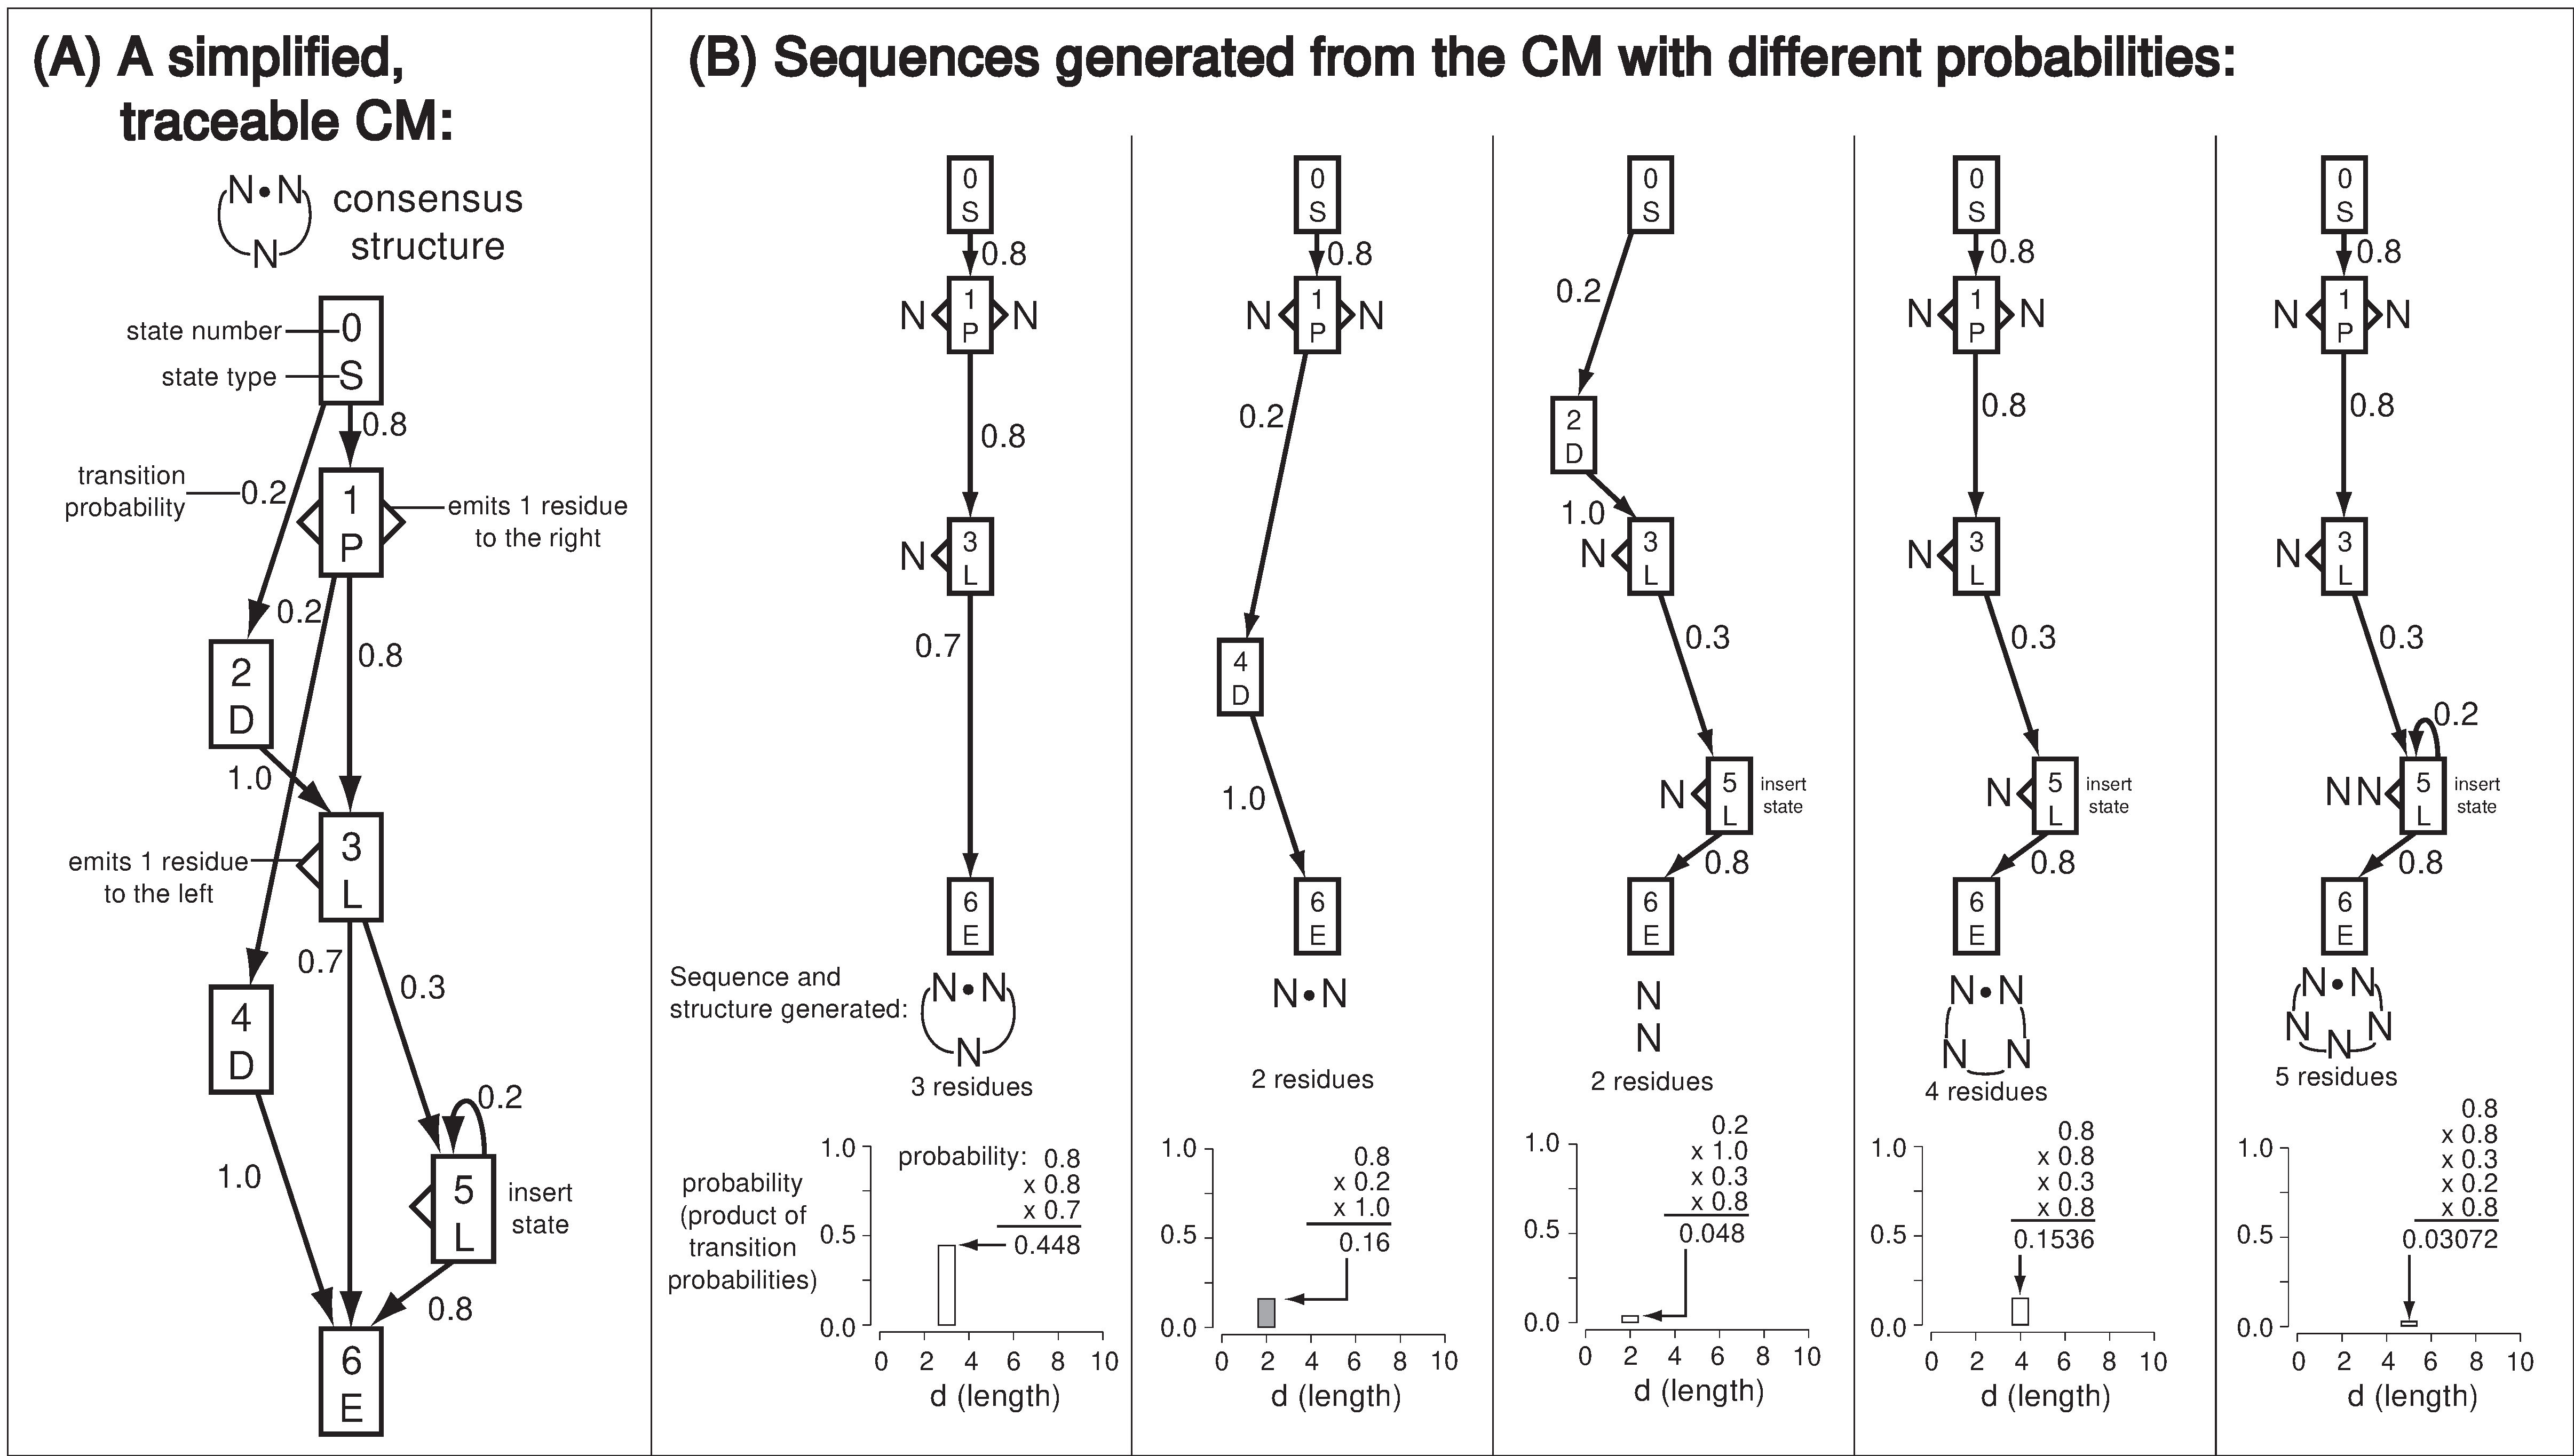
\includegraphics[width=6.4in]{figs/d3_apriori_AB}
\caption{\textbf{A simplified CM.} \textbf{(A):} Biologically
  unrealistic, toy CM with simplified architecture. \textbf{(B):} Examples of
  sequences generated from CM in (A), each with its own probability
  given the transition probabilities of the model, as shown in plots at
   bottom.}
\label{fig:aprioriAB}
\end{center}
\end{figure}
\fi

Although it is convenient to think of CMs as generative models, their
utility lies in the ability to align existing sequences and score
the alignments to predict homology. Given a parameterized model
and a sequence, the CYK dynamic programming algorithm optimally aligns
the sequence to the model by determining the most probable path
through the model that could have generated the
sequence \cite{Durbin98}. The algorithm
is easily extended to allow local alignment to the model by permitting
transitions that bypass subtree(s) of the model \cite{KleinEddy03}.

\subsection{Accelerating CM methods using a banded strategy}
The banded method we introduce accelerates CYK alignment by reducing
the number of potential paths through the model that are considered. This
technique relies on two specific features of the SCFG
architecture of CMs\@. Notably, this approach is applicable to any
probabilistic model with the following two characteristics, however we
believe it is mainly useful for SCFG methods:

\begin{description}
\item[1.] Cycles in the graph (tree) of states are restricted to emitting
  rules. 
\item[2.] With states numbered in preorder traversal, no state
  $v$ can transit to a state $y$ if $v > y$.
\end{description}

The alignment of a sequence to a CM is represented as a \emph{parse
tree} which specifies the boundaries of the subsequences that are
aligned to each subtree of the model. The CYK algorithm determines the
most likely parse tree of a sequence
given a CM by considering the alignment of all possible length
subsequences (from $0$ up to $L$, the length of the RNA)
to each subtree. Our banded strategy determines and
enforces state specific bounds on the lengths of subsequences that
are permitted to be aligned to each subtree of the model (each state
is the root of a different subtree). The bounds are implemented as
bands on the CYK dynamic programming matrix; cells outside the bands
are ignored. 
Next, considering the CM as a generative model, we present an
algorithm that determines these bands from the transition
probabilities of the model.

\subsubsection{Band calculation algorithm}
The band calculation algorithm iteratively calculates
$\gamma_v(d)$, the probability that the subtree of the model rooted at state $v$
will generate a subsequence of length $d$. This is the summed probability
of all possible paths through the subtree rooted at $v$ (i.e. paths
that start at $v$ and end at the nearest $E$ state $y > v$) that emit
exactly $d$ residues. 
The calculation initializes at the smallest subtrees ($E$ states) and
shortest subsequences ($d=0$) and iterates upwards and outwards to
progressively larger subtrees and longer subsequences. The band calculation algorithm is as follows:

\vspace{0.5em}
\begin{tabular}{l|l|l}
\multicolumn{3}{l}{for $v = M$ down to $1$:} \\
$v = $ end state $(E)$: & $\gamma_v(0) = 1$ & \\
                        & $\gamma_v(d) = 0$ & for $d=1$ to $Z$ \\
& & \\
$v = $ bifurcation $(B)$: & $\gamma_v(d) = \sum_{n=0}^{d} \gamma_y(n)
* \gamma_z(d-n)$ & for $d = 0$ to $Z$ \\
& & \\
else ($v = S, P, L, R$): & $\gamma_v(d) = 0$ & for $d=0$ to $(\Delta_v^{L} + \Delta_v^{R} -
1)$ \\
& $\gamma_v(d) = \sum_{y \in C_v} \gamma_y(d-(\Delta_v^{L} + \Delta_v^{R})) * t_v(y) $ 
& for $d = (\Delta_v^{L} + \Delta_v^{R})$ to $Z$ \\
\end{tabular}
\vspace{0.5em}

For example, if we're calculating $\gamma_v(d)$ and $v$ is
is a pair state we know that state $v$
will emit a pair of residues and transit to a new state $y$ (one
of its possible transitions $C_v$) which then will have to account for
the smaller subsequence of length $d-2$. Therefore, $\gamma_v(d)$ is
the sum, over all possible states $y$ in $C_v$, of the 
probability of transiting to $y$ ($t_v(y)$) and generating a subsequence
of length $(d-2)$ from the subtree rooted at $y$ (i.e. the
previously calculated solution $\gamma_y(d-2)$). 
For $B$ states, the algorithm uses $\gamma$ values for predefined children states $y$
and $z$.
Figure~\ref{fig:aprioriC} traces the band calculation algorithm for the simplified
CM in Figure~\ref{fig:aprioriAB}.


\ifdraft
\begin{figure}
\begin{center}
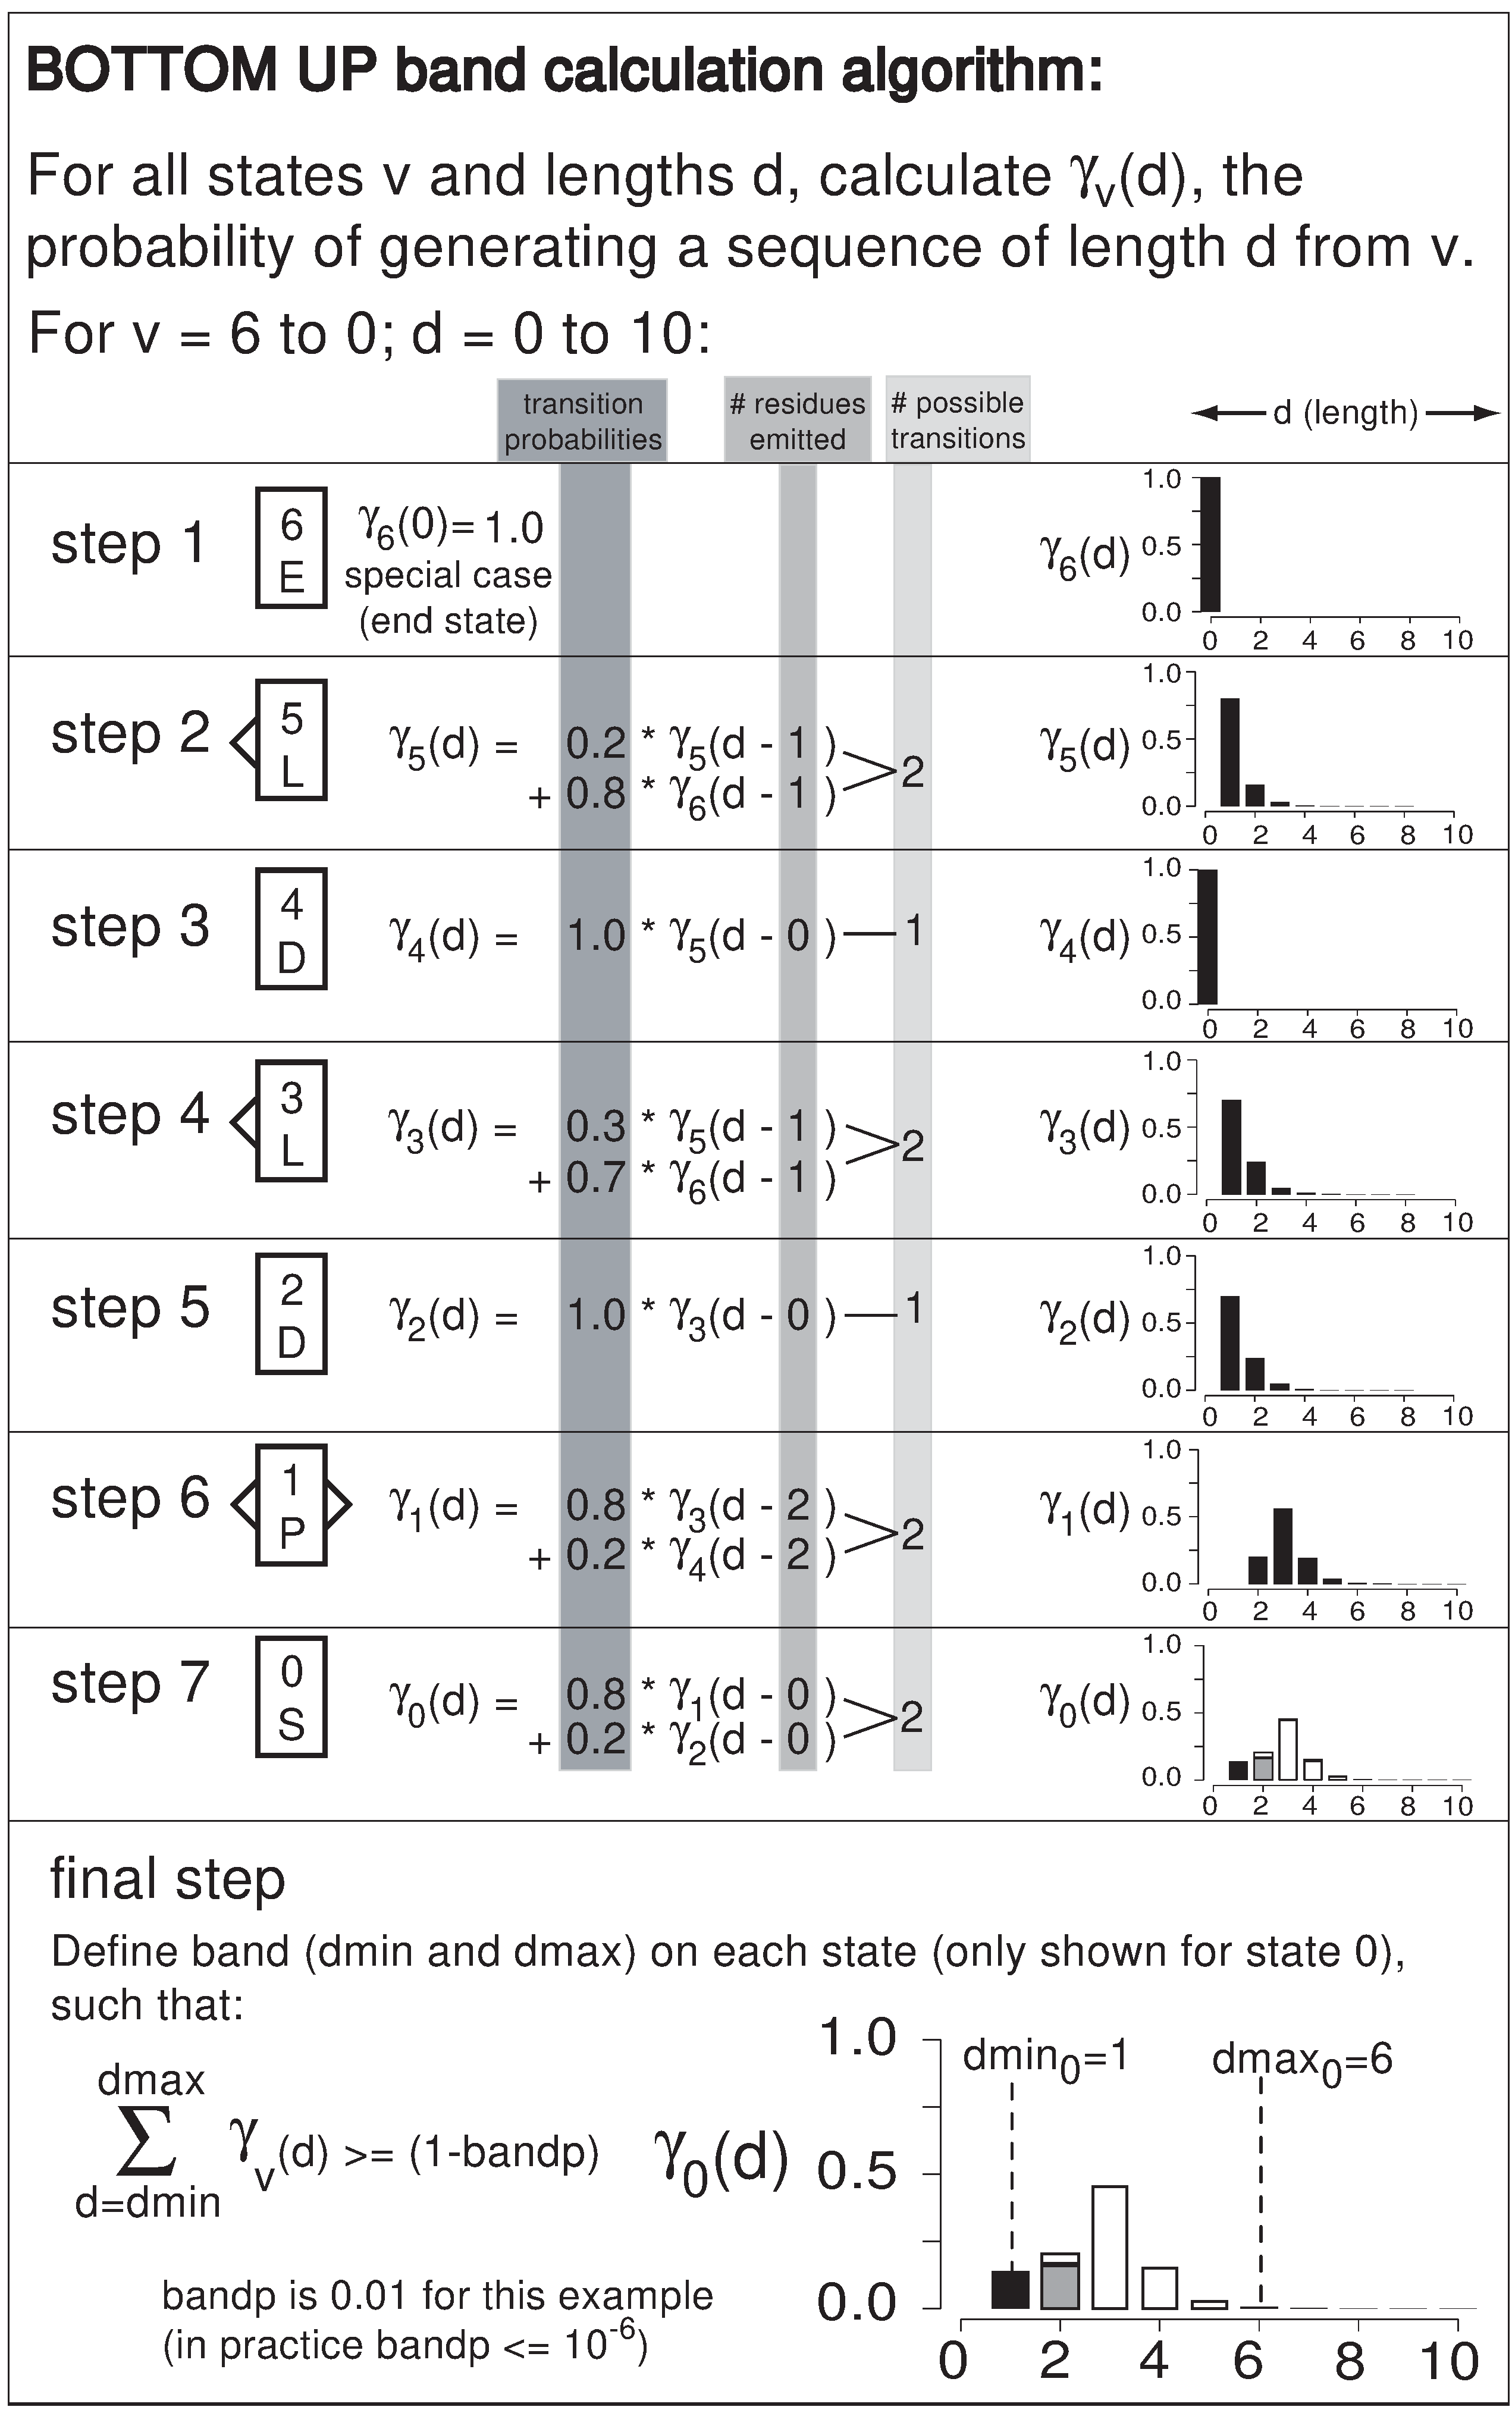
\includegraphics[width=4.5in]{figs/d3_apriori_C}
\caption{\textbf{A trace of the band calculation
  algorithm for the simplified CM in Figure~\ref{fig:aprioriAB}.} 
    The maximum length $d$ considered (the $Z$ parameter) is set as
    10. Resulting $\gamma$ probability distributions shown at right. For
    state $0$ (step 7), the $\gamma$ plot is color-coded to correspond
    with probabilities in Figure~\ref{fig:aprioriAB}.}
\label{fig:aprioriC}
\end{center}
\end{figure}
\fi

The calculation of $\gamma_v(d)$ is dependent on other $\gamma$
values. The two features of CMs previously mentioned (i.e. (1) no
non-emitting loops and (2) $v <= y$ for $y$ in $C_v$) enforce
that, when calculating $\gamma_v(d)$ all $\gamma_y$ values that
$\gamma_v(d)$ is dependent on have been previously calculated. 
Intuitively, this constraint is satisfied because the algorithm
calculates $\gamma$ values as it moves up the model to progressively
larger subtrees and longer subsequences, at each step requiring only
$\gamma$ values for shorter subsequences from states at or below the
current one. 

Bands are derived from the $\gamma$ values as follows.
The parameters $dmin_v$ and $dmax_v$ represent the minimum and maximum
allowed subsequence lengths that can be aligned to the subtree
at state $v$. These bounds are set such that: 

\[
\sum_{d = dmin_v}^{dmax_v} \gamma_v(d) \geq (1-bandp)
\]

This asserts that the probability that a subtree
rooted at state $v$ generates a subsequence of length at least
$dmin_v$ and at most $dmax_v$ is above a specified probability
threshold $(1-bandp)$. Therefore, $bandp$ is the maximum allowable
probability mass \emph{outside} the band for any state in the
model. Values of $bandp$ used are typically between $10^{-6}$ and
$10^{-10}$. 

Importantly, $\gamma_v(d)$ values are only calculated for $d$ up to a
maximum sequence length of $Z$. Because CMs have emitting self-loops
(i.e. insert states), there is no limit to the length of a sequence
that can be generated from (i.e. aligned to) any subtree of the model
that includes an insert state. However, calculation of the
$\gamma$ values neglect the probability that a subsequence
of length $d > Z$ will be generated by any subtree.
Therefore, $Z$ must be sufficiently large such that the cumulative
probability of all such subsequences is ``negligible''. Our
implementation handles this by enforcing that this cumulative
probability is very small (?).

\subsubsection{Using the band calculation to determine the maximum
  size of a hit to a CM}
The $W$ parameter is used during database search with CMs to
define the maximum size of a hit to a model. Previous implementations
required that the $W$ parameter be manually set by the user. 
The band calculation algorithm delivers a probabilistically derived
$W$ for database search in $dmax_0$, which is the upper bound on the
length of the entire sequence (the sequence generated by the top-most
state, the root of the entire tree). 

\subsubsection{The banded CYK database search algorithm}
%The CM CYK database search algorithm is used to find subsequences of
%long sequences (i.e. chromosomes) that align with high scores to the
%CM, and are therefore likely homologs of the family being
%modelled. 
Th CM CYK database search algorithm is different from the traditional
CYK algorithm \cite{Kasami65, Younger67, HopcroftUllman79} in several
important respects. First, while the traditional CYK is used with
Chomsky normal form (CNF) grammars, the CM CYK is specially adapted
for the CM grammar, which is not CNF\@. Secondly, CM CYK does not find
the optimal parse tree of the entire input sequence, but
rather scans the sequence and finds the set of
non-overlapping subsequences (hits) that each align globally with
respect to the model for which the summed score is maximized. Finally, 
transformed coordinates are used to allow a simple, memory efficient
implementation of the scanning algorithm. Specifically, instead of the
traditional $i$ and $j$ CYK coordinates for subsequence begin and end
positions respectively, the CM CYK uses $j$ and $d$ coordinates with
$d = j-i+1$ \cite{Durbin98}.

The CM CYK search algorithm calculates $\alpha_v(j,d)$ - the log odds score
of the most likely CM parse subtree rooted at state $v$ that generates
(aligns to) the length $d$ subsequence $x_{j-d+1}..x_j$ of sequence
$x$ \cite{Durbin98}. 
Similar to the band calculation algorithm, this calculation initializes
at the smallest subtrees ($E$ states) and shortest subsequences
($d=0$) and iterates upward and outward to progressively larger
subtrees and longer subsequences. 

We accelerate CYK database search using bands ($dmin$ and $dmax$
values) derived from the band calculation algorithm. The bands
correspond to state specific bounds on the $d$ dimension of the
$\alpha$ matrix that limit possible values of $d$ (subsequence
lengths) that can be aligned to each subtree of the model. The bands
are applied by initializing all cells of the matrix outside the bands
to a score of $-\infty$, and never
reevaluating them during the recursion. The banded CYK database search
algorithm is: 

%CYK for CM database search - banded version (ref p.290 Durbin)
\vspace{0.5em}
\begin{tabular}{l|l}
\multicolumn{2}{l}{Initialization (impose bands): for $j = 0$ to $L$,
  $v = M$ down to $1$:} \\
for $d = 0$ to $\min((dmin_v-1), j)$ & $\alpha_v(j,d) = -\infty;$ \\
for $d = (dmax_v+1)$ down to $j$ & $\alpha_v(j,d) = -\infty;$ \\
& \\
\multicolumn{2}{l}{Initialization at $d = 0$: for $j = 0$ to $L$,
$v = M$ down to $1$:} \\
$v = $ end state $(E)$: & $\alpha_v(j,0) = 0$ \\
$v = $ bifurcation $(B)$: & $\alpha_v(j,0) = \alpha_y(j,0) +
\alpha_z(j,0)$ \\
$v = $ delete or start $(D,S)$: & $\alpha_v(j,0) = \max_{y \in C_v} [\alpha_y(j,0) +
  \log t_v(y)];$ \\
else $(v=P,L,R)$ & $\alpha_v(j,0) = -\infty$ \\
& \\
\multicolumn{2}{l}{Recursion: for $j = 1$ to $L, d = max(1,dmin_v)$ to
  $min(dmax_v,j), v=M$ down to $1$} \\
$v = $ end state $(E)$: & $\alpha_v(j,d) = - \infty$ \\
$v = $ bifurcation $(B)$: & $kmin = max(dmin_z, (d-dmax_y))$ \\
& $kmax = min(dmax_z, (d-dmin_y))$ \\
& $\alpha_v(j,d) = \max_{kmin \le k \le kmax}[\alpha_y(j-k,d-k) +
    \alpha_z(j,k)];$ \\
$v = $ delete or start $(D,S)$: & $\alpha_v(j,d) = \max_{y \in C_v} [\alpha_y(j,d) +
  \log t_v(y)];$ \\
else $(v = P, L, R):$ & $\alpha_v(j,d) = \max_{y \in C_v}
  [\alpha_y(j-\Delta_v^{R}, d-(\Delta_v^{L}+\Delta_v^{R})) + \log
  t_v(y)]$ \\
& \hspace{4.5em} $+ \log e_v(x_i,x_j)$ \\ 
\end{tabular}
\vspace{0.5em}

For example, if we're calculating $\alpha_v(j,d)$ and 
$v$ is a pair state ($P$), $v$ will generate the basepair $x_{j-d+1},x_j$ and
transit to a new state $y$ (one of its possible transitions $C_v$)
which then will have to account for the smaller subsequence
$x_{j-d+2}..x_{j-1}$. The log odds score for a particular choice of
next state $y$ is the sum of three terms: an emission term $\log
e_v(x_{j-d+1},x_j)$, a transition term $\log t_v(y)$, and an already
calculated solution for the smaller optimal parse tree rooted at $y$,
$\alpha_y(j-1,d-2)$. The value assigned to $\alpha_v(j, d)$
is the maximum over all possible choices of child states $y$ that $v$
can transit to. 

\subsection{Tuning speed versus accuracy with the $bandp$ parameter}
The banded CM CYK algorithm offers acceleration by ignoring all
alignments that violate the band of at least one state, and finds
the optimal alignment consistent with all the bands. Therefore, when
the globally optimal solution is not consistent with the bands, the
acceleration comes at a cost to sensitivity. This is most likely to
occur when aligning remote homologs, which may have significantly
different subsequence lengths in some homologous regions. This 
speed versus
accuracy tradeoff can be controlled to an extent by the $bandp$
parameter. In general, higher $bandp$ values will give tighter bands
that result in faster, less sensitive searches than lower $bandp$ values.
Empirically, practical values of $bandp$ are between $10^{-6}$ and
$10^{-10}$ (see benchmark results). 

\subsection{Informative transition priors for appropriate band calculation}

The band calculation algorithm uses only the transition probabilities
of the model to determine the bands. These probabilities are
themselves calculated as mean posterior estimates using
observed counts from the input alignment and a Dirichlet prior
\cite{infguide03}. Previous to this work, uninformative Dirichlet
densities corresponding to Laplace ``plus-1'' pseudo-counts were used
as transition priors. However, uninformative priors are
problematic during band calculation because they do not accurately
reflect the distributions that would be observed from actual RNA
sequences, and result in inappropriate bands that would often ignore
the optimal alignment.  This problem is exacerbated when there are few
training sequences, because the prior has more of an impact during
mean posterior estimation. 
Figure~\ref{fig:3bands} depicts the effect of plus-1 priors on band
calculation anecdotally for three RNA families by showing that the
the bounds on the full length of potential new homologs ($dmin_0$ and $dmax_0$)
do not appropriately reflect the lengths of the sequences
in the input alignment. 

\ifdraft
\begin{figure}
  \label{fig:3bands}
  \begin{center}
    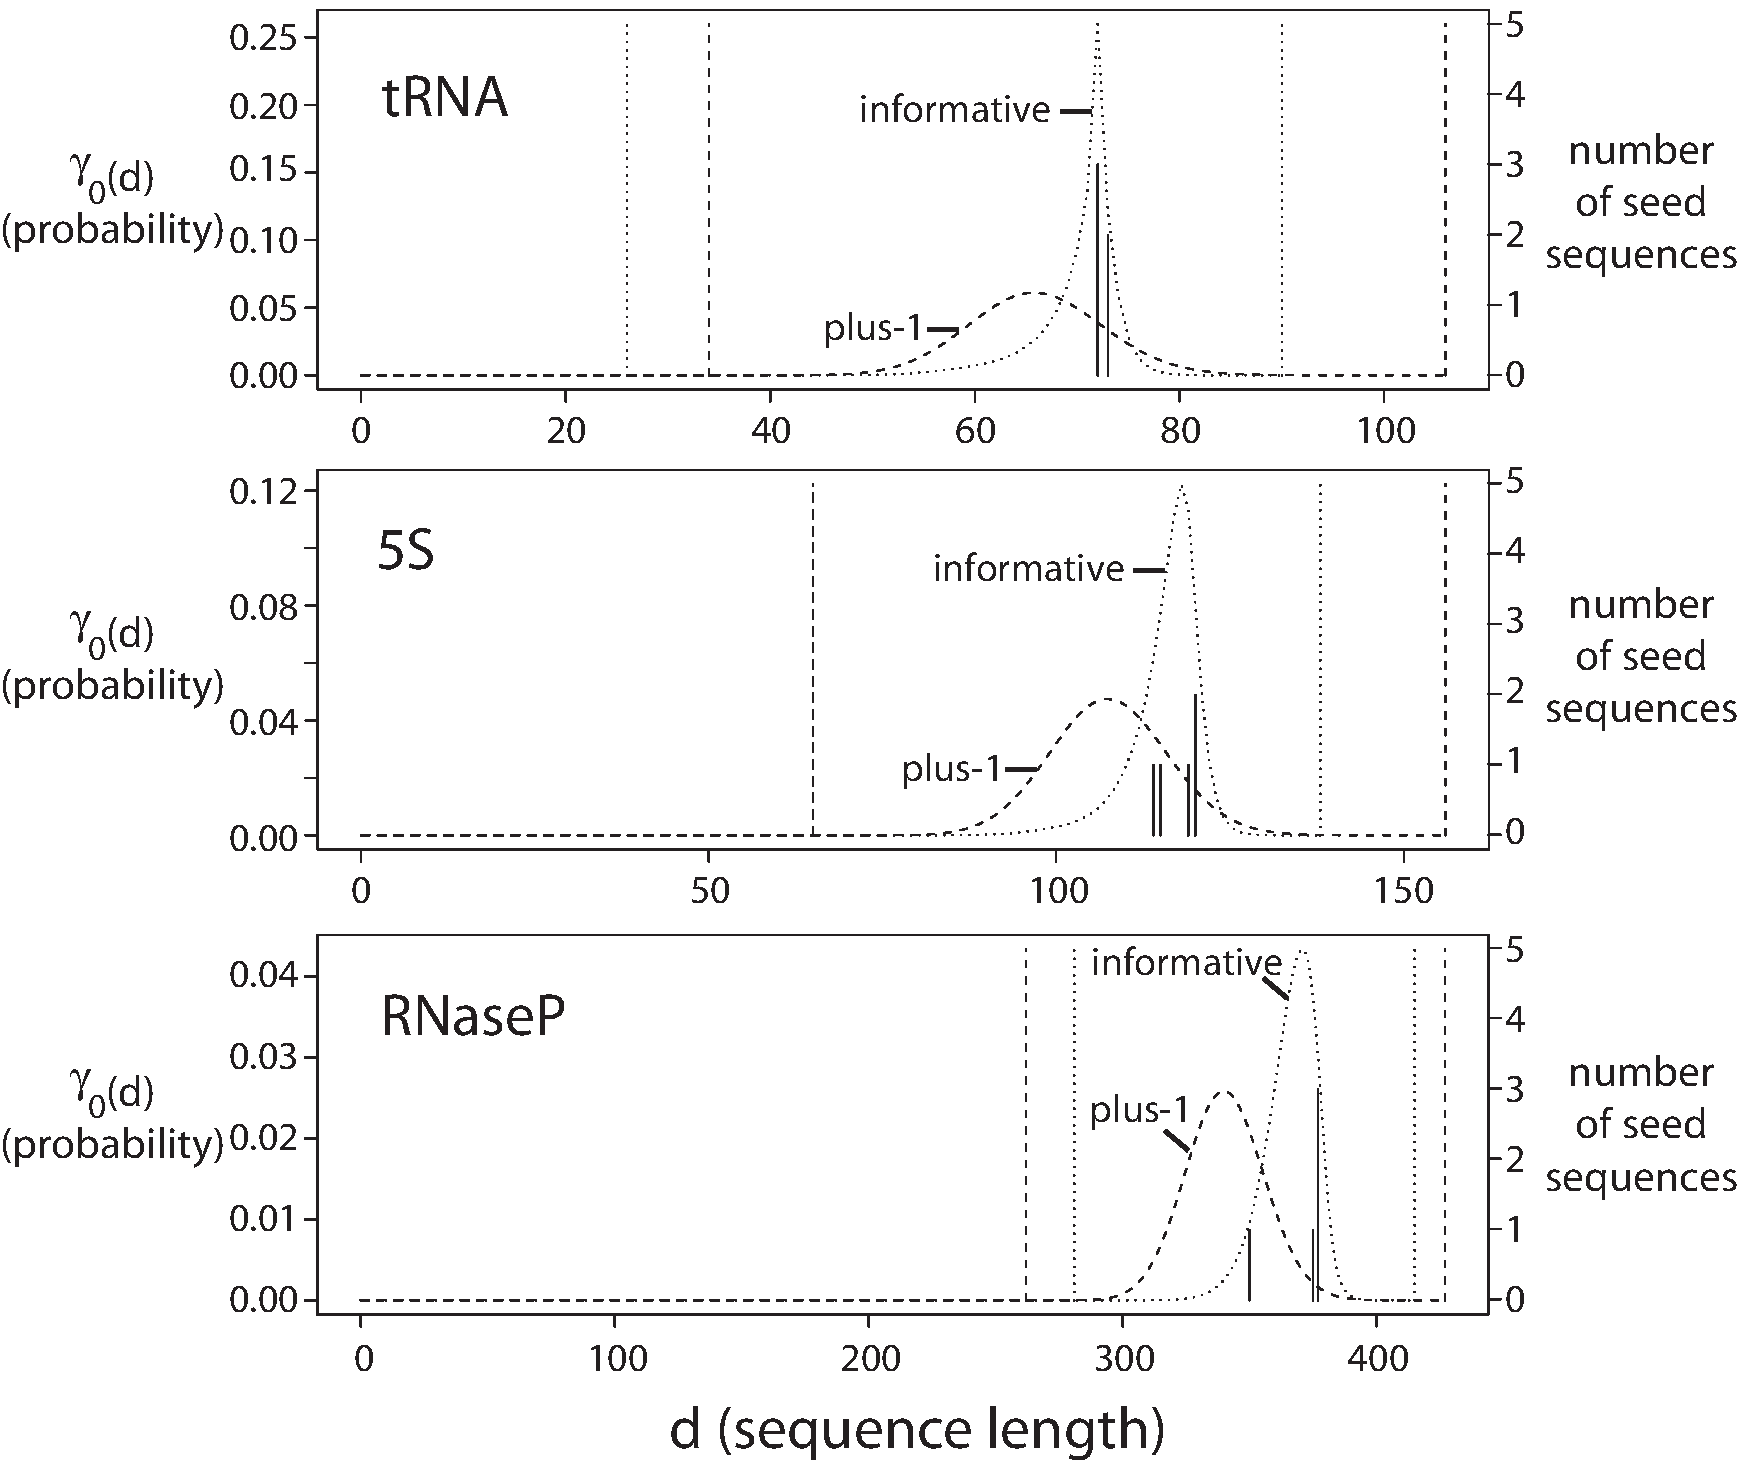
\includegraphics[width=6in,angle=0]{figs/3fam_bands}
    \caption{\textbf{Effect of transition priors on band calculation.}
      Solid vertical lines represent the lengths of the 5
      training sequences in the alignment used to build each model,
      corresponding with the
      right vertical axis labels. Band calculation is compared using
      ``plus-1'' transition priors and the newly estimated ``informative''
      Dirichlet priors as follows: Dashed
      probability distributions show $\gamma_0(d)$, the probability a
      sequence of length $d$ is generated by (i.e. will be aligned to)
      state $0$ (the top-most, root state)
      of each model. Dashed vertical lines indicate the band values
      ($dmin_0$ (left) and
      $dmax_0$ (right)) derived from the $\gamma_0(d)$ distribution using $bandp =
      10^{-7}$ (the probability mass within each band is 99.99999\%).}
  \end{center}
\end{figure}
\fi

To alleviate this problem, we estimated many (36) single component Dirichlet
densities to be used as informative transition priors that accurately
reflect characteristics of RNA sequences. The specific density used as
a prior for mean posterior estimation of transition probabilities out
of a given state $v$ to potential states $C_v$ is dependent on the node and
state types of the states in $C_v$. The CM architecture allows exactly
73 possible ``transition alphabets'' of node and state types in
$C_v$. Instead of estimating 73 Dirichlet densities, we defined 36
groups of transition alphabets by combining similar alphabets into the
same group, and estimated a Dirichlet density for each group to be
applied for all alphabets in the group. We derived training data for
estimatiion of the Dirichlet densities from version 6.1 of the Rfam
database \cite{Griffiths-Jones05}.
Specifically, we built CMs from each of the 381 Rfam version 6.1 seed
alignments and collected counts of the
observed transitions used in the parse trees of each seed sequence.
Table~\ref{tbl:transitions} contains statistics on the counts collected
for each of the transition alphabets and groups of alphabets.
%Using this training data, a Dirichlet density was estimated for each
%to be applied to all transition alphabets in that group. 
Dirichlet densities were estimated from these counts using the maximum
likelihood based method described in \cite{Sjolander96} with one
exception, our procedure used a conjugate gradient descent algorithm
\cite{Press93} for optimization while \cite{Sjolander96} describes an
expectation-maximization (EM) based approach.  The resulting Dirichlet
parameters are in Table~\ref{tbl:transitions}.  
%For exactly six alphabets
%comprising three groups, the number of count vectors was so low ($\le
%2$) we decided to continue use of plus-1 priors (these are marked by
%* in Table~\ref{tbl:transitions}).  
Incorporating the informative transition priors during mean posterior
estimation of the transition probabilities has a dramatic impact
on calculation of the bands as shown in Figure~\ref{fig:3bands}.

% The transition priors 041006_trans_priors.tex (with modifications)
\ifdraft
\renewcommand{\baselinestretch}{1.0}
\begin{table}
\renewcommand{\tabcolsep}{0.7em}
\tiny
\begin{center}
%\begin{tabular}{|r|r|l|l|l||l|r||l|r||l|r||l|r||l|r||l|r||} \hline
\begin{tabular}{|rr|rr|cc|c|c|cc|cc|cc|cc|cc|cc|} \cline{1-6} \cline{8-20}
%\multicolumn{5}{c}{} & \multicolumn{2}{|c|}{1} & \multicolumn{2}{|c|}{2} & \multicolumn{2}{|c|}{3} & \multicolumn{2}{|c|}{4} & \multicolumn{2}{|c|}{5} & \multicolumn{2}{|c|}{6} \\ \cline{1-17}
\multicolumn{1}{|c}{alph} & \multicolumn{1}{c|}{grp} &
  \multicolumn{1}{c}{alph} & \multicolumn{1}{c|}{grp} & node & next &
  & \multicolumn{13}{|c|}{transition alphabets and Dirichlet $\alpha$ parameters} \\ %\cline{8-20}
%\multicolumn{1}{|c}{\#} & \multicolumn{1}{c|}{\#} & \multicolumn{1}{c}{counts} & \multicolumn{1}{c|}{counts} & state & node & & $|\alpha|$ & $a_1$ &
%  $\frac{\alpha_{a_1}}{|\alpha|}$ & $a_2$ & $\frac{\alpha_{a_2}}{|\alpha|}$ & $a_3$ &
%  $\frac{\alpha_{a_3}}{|\alpha|}$ & $a_4$ & $\frac{\alpha_{a_4}}{|\alpha|}$ & $a_5$ &
%  $\frac{\alpha_{a_5}}{|\alpha|}$ & $a_6$ & $\frac{\alpha_{a_6}}{|\alpha|}$ \\
%  \cline{1-6} \cline {8-20} 
\multicolumn{1}{|c}{\#} & \multicolumn{1}{c|}{\#} & \multicolumn{1}{c}{counts} & \multicolumn{1}{c|}{counts} & state & node & & $|\alpha|$ & $a$ &
  $\frac{\alpha_{a}}{|\alpha|}$ & $a$ & $\frac{\alpha_{a}}{|\alpha|}$ & $a$ &
  $\frac{\alpha_{a}}{|\alpha|}$ & $a$ & $\frac{\alpha_{a}}{|\alpha|}$ & $a$ &
  $\frac{\alpha_{a}}{|\alpha|}$ & $a$ & $\frac{\alpha_{a}}{|\alpha|}$ \\
  \cline{1-6} \cline {8-20} 

1   &    & 6     & 11    & MATP\_MP & BIF  & & 0.5509  & IL & 0.1229 & IR & 0.0001 & B  & 0.8770 &    &        &    &  &  &  \\  
2   &    & 7023  & 7119  & MATP\_MP & MATP & & 7.2986  & IL & 0.0023 & IR & 0.0024 & MP & 0.9816 & ML & 0.0056 & MR & 0.0046 & D & 0.0035 \\  
3   &    & 1600  & 1830  & MATP\_MP & MATL & & 1.5914  & IL & 0.0179 & IR & 0.0155 & ML & 0.9200 & D  & 0.0466 &    &  &  &  \\  
4   &    & 145   & 195   & MATP\_MP & MATR & & 1.9038  & IL & 0.0173 & IR & 0.0073 & MR & 0.8903 & D  & 0.0852 &    &  &  &  \\  
5   & 1  & 2     & 11    & MATP\_MP & END  & & 0.5509  & IL & 0.1229 & IR & 0.0001 & E  & 0.8770 &    &        &    &  &  &  \\  
6*  &    & 1     & 2     & MATP\_ML & BIF  & & 3.0000  & IL & 0.3333 & IR & 0.3333 & B  & 0.3333 &    &        &    &  &  &  \\  
7   &    & 577   & 577   & MATP\_ML & MATP & & 0.6941  & IL & 0.0131 & IR & 0.0103 & MP & 0.4032 & ML & 0.4983 & MR & 0.0115 & D & 0.0636 \\  
8   &    & 133   & 133   & MATP\_ML & MATL & & 0.9316  & IL & 0.0739 & IR & 0.0651 & ML & 0.7038 & D  & 0.1571 &    &  &  &  \\  
9   &    & 15    & 15    & MATP\_ML & MATR & & 0.3272  & IL & 0.1884 & IR & 0.0432 & MR & 0.4082 & D  & 0.3602 &    &  &  &  \\  
10* & 6  & 1     & 2     & MATP\_ML & END  & & 3.0000  & IL & 0.3333 & IR & 0.3333 & E  & 0.3333 &    &        &    &  &  &  \\  
11* &    & 1     & 2     & MATP\_MR & BIF  & & 3.0000  & IL & 0.3333 & IR & 0.3333 & B  & 0.3333 &    &        &    &  &  &  \\  
12  &    & 531   & 531   & MATP\_MR & MATP & & 0.7987  & IL & 0.0079 & IR & 0.0190 & MP & 0.3241 & ML & 0.0193 & MR & 0.5631 & D & 0.0666 \\  
13  &    & 151   & 151   & MATP\_MR & MATL & & 0.6933  & IL & 0.0357 & IR & 0.0699 & ML & 0.3066 & D  & 0.5879 &    &  &  &  \\  
14  &    & 15    & 15    & MATP\_MR & MATR & & 0.3574  & IL & 0.0582 & IR & 0.0002 & MR & 0.7629 & D  & 0.1787 &    &  &  &  \\  
15* & 11 & 1     & 2     & MATP\_MR & END  & & 3.0000  & IL & 0.3333 & IR & 0.3333 & E  & 0.3333 &    &        &    &  &  &  \\  
16* &    & 0     & 2     & MATP\_D  & BIF  & & 3.0000  & IL & 0.3333 & IR & 0.3333 & B  & 0.3333 &    &        &    &  &  &  \\  
17  &    & 575   & 575   & MATP\_D  & MATP & & 0.5450  & IL & 0.0019 & IR & 0.0047 & MP & 0.0857 & ML & 0.0534 & MR & 0.0528 & D & 0.8015 \\  
18  &    & 149   & 149   & MATP\_D  & MATL & & 0.5831  & IL & 0.0421 & IR & 0.0526 & ML & 0.2080 & D  & 0.6973 &    &  &  &  \\  
19  &    & 14    & 14    & MATP\_D  & MATR & & 0.1164  & IL & 0.0001 & IR & 0.0001 & MR & 0.2439 & D  & 0.7559 &    &  &  &  \\  
20* & 16 & 2     & 2     & MATP\_D  & END  & & 3.0000  & IL & 0.3333 & IR & 0.3333 & E  & 0.3333 &    &        &    &  &  &  \\  
21  &    & 2     & 4     & MATP\_IL & BIF  & & 1.4397  & IL & 0.6553 & IR & 0.0445 & B  & 0.3002 &    &        &    &  &  &  \\  
22  &    & 121   & 126   & MATP\_IL & MATP & & 0.9402  & IL & 0.1673 & IR & 0.1394 & MP & 0.5904 & ML & 0.0443 & MR & 0.0259 & D & 0.0327 \\  
23  &    & 114   & 119   & MATP\_IL & MATL & & 0.8046  & IL & 0.3108 & IR & 0.1936 & ML & 0.4610 & D  & 0.0346 &    &  &  &  \\  
24  &    & 14    & 15    & MATP\_IL & MATR & & 1.0926  & IL & 0.1419 & IR & 0.0501 & MR & 0.6538 & D  & 0.1541 &    &  &  &  \\  
25  & 21 & 2     & 4     & MATP\_IL & END  & & 1.4397  & IL & 0.6553 & IR & 0.0445 & E  & 0.3002 &    &        &    &  &  &  \\  
26  &    & 1     & 31    & MATP\_IR & BIF  & & 0.9361  & IR & 0.2827 & B  & 0.7173 &    &        &    &        &    &  &  &  \\  
27  &    & 145   & 227   & MATP\_IR & MATP & & 1.5494  & IR & 0.1884 & MP & 0.7090 & ML & 0.0165 & MR & 0.0588 & D  & 0.0273 &  &  \\  
28  &    & 129   & 701   & MATP\_IR & MATL & & 1.6332  & IR & 0.3681 & ML & 0.5752 & D  & 0.0566 &    &        &    &  &  &  \\  
29  &    & 8     & 160   & MATP\_IR & MATR & & 1.2428  & IR & 0.2633 & MR & 0.6809 & D  & 0.0558 &    &        &    &  &  &  \\  
30  & 26 & 0     & 31    & MATP\_IR & END  & & 0.9361  & IR & 0.2827 & E  & 0.7173 &    &        &    &        &    &  &  &  \\  
31  &    & 108   & 1130  & MATL\_ML & BIF  & & 1.2298  & IL & 0.0078 & B  & 0.9922 &    &        &    &        &    &  &  &  \\  
32  &    & 420   & 1319  & MATL\_ML & MATP & & 2.4162  & IL & 0.0132 & MP & 0.9520 & ML & 0.0150 & MR & 0.0129 & D  & 0.0070 &  &  \\  
33  &    & 19013 & 19371 & MATL\_ML & MATL & & 1.8632  & IL & 0.0082 & ML & 0.9711 & D  & 0.0207 &    &        &    &  &  &  \\  
34  &    & 859   & 6692  & MATL\_ML & MATR & & 72.1283 & IL & 0.0058 & MR & 0.9755 & D  & 0.0187 &    &        &    &  &  &  \\  
35  & 31 & 801   & 1130  & MATL\_ML & END  & & 1.2298  & IL & 0.0078 & E  & 0.9922 &    &        &    &        &    &  &  &  \\  
36  &    & 28    & 172   & MATL\_D  & BIF  & & 6.8008  & IL & 0.0029 & B  & 0.9971 &    &        &    &        &    &  &  &  \\  
37  &    & 103   & 103   & MATL\_D  & MATP & & 0.7288  & IL & 0.0321 & MP & 0.5730 & ML & 0.0536 & MR & 0.1654 & D  & 0.1758 &  &  \\  
38  &    & 3152  & 3152  & MATL\_D  & MATL & & 0.4101  & IL & 0.0138 & ML & 0.3105 & D  & 0.6756 &    &        &    &  &  &  \\  
39  &    & 154   & 154   & MATL\_D  & MATR & & 0.6736  & IL & 0.0203 & MR & 0.6014 & D  & 0.3782 &    &        &    &  &  &  \\  
40  & 36 & 144   & 172   & MATL\_D  & END  & & 6.8008  & IL & 0.0029 & E  & 0.9971 &    &        &    &        &    &  &  &  \\  
41  & 26 & 13    & 31    & MATL\_IL & BIF  & & 0.9361  & IL & 0.2827 & B  & 0.7173 &    &        &    &        &    &  &  &  \\  
42  & 27 & 35    & 227   & MATL\_IL & MATP & & 1.5494  & IL & 0.1884 & MP & 0.7090 & ML & 0.0588 & MR & 0.0165 & D  & 0.0273 &  &  \\  
43  & 28 & 549   & 701   & MATL\_IL & MATL & & 1.6332  & IL & 0.3681 & ML & 0.5752 & D  & 0.0566 &    &        &    &  &  &  \\  
44  & 29 & 45    & 160   & MATL\_IL & MATR & & 1.2428  & IL & 0.2633 & MR & 0.6809 & D  & 0.0558 &    &        &    &  &  &  \\  
45  & 26 & 0     & 31    & MATL\_IL & END  & & 0.9361  & IL & 0.2827 & E  & 0.7173 &    &        &    &        &    &  &  &  \\  
46  & 31 & 206   & 1130  & MATR\_MR & BIF  & & 1.2298  & IR & 0.0078 & B  & 0.9922 &    &        &    &        &    &  &  &  \\  
47  & 32 & 848   & 1319  & MATR\_MR & MATP & & 2.4162  & IR & 0.0132 & MP & 0.9520 & ML & 0.0150 & MR & 0.0129 & D  & 0.0070 &  &  \\  
48  & 34 & 5833  & 6692  & MATR\_MR & MATR & & 2.1283  & IR & 0.0058 & MR & 0.9755 & D  & 0.0187 &    &        &    &  &  &  \\  
49  &    & 39    & 39    & MATR\_D  & BIF  & & 0.4664  & IR & 0.0463 & B  & 0.9537 &    &        &    &        &    &  &  &  \\  
50  &    & 176   & 176   & MATR\_D  & MATP & & 0.8689  & IR & 0.0245 & MP & 0.6126 & ML & 0.1269 & MR & 0.0471 & D  & 0.1890 &  &  \\  
51  &    & 771   & 771   & MATR\_D  & MATR & & 0.4869  & IR & 0.0119 & MR & 0.3373 & D  & 0.6507 &    &        &    &  &  &  \\  
52  & 26 & 15    & 31    & MATR\_IR & BIF  & & 0.9361  & IR & 0.2827 & B  & 0.7173 &    &        &    &        &    &   &  &  \\  
53  & 27 & 39    & 227   & MATR\_IR & MATP & & 1.5494  & IR & 0.1884 & MP & 0.7090 & ML & 0.0165 & MR & 0.0588 & D  & 0.0273 &  &  \\  
54  & 29 & 107   & 160   & MATR\_IR & MATR & & 1.2428  & IR & 0.2633 & MR & 0.6809 & D  & 0.0558 &    &        &    &  &  &  \\  
%55 &    &       &       & BEGL\_S  & BIF  & & 1.0000  & B  & 1.0000 &    &        &    &        &    &        &    &  &  &  \\  
55  &    & 338   & 338   & BEGL\_S  & MATP & & 5.0422  & MP & 0.9579 & ML & 0.0121 & MR & 0.0183 & D  & 0.0117 &    &   &  &  \\  
56  & 31 & 15    & 1130  & BEGR\_S  & BIF  & & 1.2298  & IL & 0.0078 & B  & 0.9922 &    &        &    &        &    &  &  &  \\  
57  & 32 & 51    & 1319  & BEGR\_S  & MATP & & 2.4162  & IL & 0.0132 & MP & 0.9520 & ML & 0.0150 & MR & 0.0129 & D  & 0.0070 &  &  \\  
58  & 33 & 358   & 19371 & BEGR\_S  & MATL & & 1.8632  & IL & 0.0082 & ML & 0.9711 & D  & 0.0207 &    &        &    &  &  &  \\  
59  & 26 & 2     & 31    & BEGR\_IL & BIF  & & 0.9361  & IL & 0.2827 & B  & 0.7173 &    &        &    &        &    &   &  &  \\  
60  & 27 & 3     & 227   & BEGR\_IL & MATP & & 1.5494  & IL & 0.1884 & MP & 0.7090 & ML & 0.0588 & MR & 0.0165 & D  & 0.0273 &  &  \\  
61  & 28 & 19    & 701   & BEGR\_IL & MATL & & 1.6332  & IL & 0.3681 & ML & 0.5752 & D  & 0.0566 &    &        &    &  &  &  \\  
62  & 1  & 3     & 11    & ROOT\_S  & BIF  & & 0.5509  & IL & 0.1229 & IR & 0.0001 & B  & 0.8770 &    &        &    &  &  &  \\  
63  & 2  & 96    & 7119  & ROOT\_S  & MATP & & 7.2986  & IL & 0.0023 & IR & 0.0024 & MP & 0.9816 & ML & 0.0056 & MR & 0.0046 & D & 0.0035 \\  
64  & 3  & 230   & 1830  & ROOT\_S  & MATL & & 1.5914  & IL & 0.0179 & IR & 0.0155 & ML & 0.9200 & D  & 0.0466 &    &  &  &  \\  
65  & 4  & 50    & 195   & ROOT\_S  & MATR & & 1.9038  & IL & 0.0173 & IR & 0.0073 & MR & 0.8903 & D  & 0.0852 &    &  &  &  \\  
66  & 21 & 0     & 4     & ROOT\_IL & BIF  & & 1.4397  & IL & 0.6553 & IR & 0.0445 & B  & 0.3002 &    &        &    &  &  &  \\  
67  & 22 & 5     & 126   & ROOT\_IL & MATP & & 0.9402  & IL & 0.1673 & IR & 0.1394 & MP & 0.5904 & ML & 0.0443 & MR & 0.0259 & D & 0.0327 \\  
68  & 23 & 5     & 119   & ROOT\_IL & MATL & & 0.8046  & IL & 0.3108 & IR & 0.1936 & ML & 0.4610 & D  & 0.0346 &    &  &  &  \\  
69  & 24 & 1     & 15    & ROOT\_IL & MATR & & 1.0926  & IL & 0.1419 & IR & 0.0501 & MR & 0.6538 & D  & 0.1541 &    &  &  &  \\  
70  & 26 & 0     & 31    & ROOT\_IR & BIF  & & 0.9361  & IR & 0.2827 & B  & 0.7173 &    &        &    &        &    &  &  &  \\  
71  & 27 & 5     & 227   & ROOT\_IR & MATP & & 1.5494  & IR & 0.1884 & MP & 0.7090 & ML & 0.0165 & MR & 0.0588 & D  & 0.0273 &  &  \\  
72  & 28 & 4     & 701   & ROOT\_IR & MATL & & 1.6332  & IR & 0.3681 & ML & 0.5752 & D  & 0.0566 &    &        &    &  &  &  \\  
73  & 29 & 0     & 160   & ROOT\_IR & MATR & & 1.2428  & IR & 0.2633 & MR & 0.6809 & D  & 0.0558 &    &        &    &  &  &  \\   \cline{1-6} \cline {8-20} 
\end{tabular}
\end{center}

\normalfont\rmfamily
\caption{\textbf{Transition alphabets and groups with corresponding
    training counts and estimated Dirichlet transition prior parameters.}
  ``alph \#''= transition alphabet number; ``*'' indicates a plus-1
  prior is used. ``grp \#''= transition
  group number, each group is numbered as the lowest numbered alphabet in
  the group, this column is blank if alphabet number = group
  number. ``alph counts''= observed Rfam 6.1 counts for
  alphabet. ``grp counts''= total Rfam 6.1 counts for group, used
  to estimate a single component Dirichlet density for use as a prior
  for each alphabet in the group. ``node state''= initial node state
  type for each alphabet. ``next node''= type of immediately downstream
  node for each alphabet.}

\label{tbl:transitions}
\end{table}
\renewcommand{\baselinestretch}{1.5}
\fi

\subsection{Increasing sensitivity by refining CM parameterization}
\subsubsection{Informative emission priors}
To complement the informative transition priors, Dirichlet density
\emph{mixtures} were estimated to use as informative emission
priors. Although the emission probabilities do not affect band calculation,
using Dirichlet density mixtures has been shown to improve the ability
of profile HMMs to detect remote protein homology \cite{Brown93b,
Sjolander96}, and we hoped to show a similar effect for CMs. 

For emission prior estimation, observed counts of single-stranded and
base-paired residues were collected from the individually structurally
annotated ribosomal RNA alignments from the European Ribosomal RNA Database
\cite{VandePeer00, Wuyts01}. Starting with four alignments
from the 2002 version of the database, sequences were removed in which either less than 40\%
of the base paired positions are present or more than 5\% of the
nucleotides are ambiguous. Each resulting alignment was filtered so
that no two sequences in a filtered alignment were greater than 80\%
identical. Characteristics of the filtered alignments and collected
counts are in Table~\ref{tbl:emissioncounts}.

%%%%%%%%%%%%%%%%%%%%%%%%%%%%%%%%%%%%%%%%%%%%%%%%%%%%%%%%%%%%%%%%%%%%%%%
% The emission prior alignment counts
% this table is in my rotation lab presentation ./emit_priors_revisited/nawrocki_dirichlet.pdf
%\renewcommand{\baselinestretch}{1.0}
\ifdraft
\begin{table}
%\normalfont\ttfamily
\begin{center}
\begin{tabular}{lrrrrrrr} 
& & \# aln & \# filtered & \# consensus & \# consensus & bp & SS \\
alignment & \# seq & columns & seq & bp & SS columns & counts & counts \\ \hline
LSU & 1551 & 7270 & 139 & 601 & 1532 & 65229 & 180558  \\
SSU bap & 12773 & 2653 & 254 & 421 & 680 & 97834 & 153565 \\
SSU euk & 7151 & 4558 & 207 & 407 & 959 & 72521 & 174260 \\
SSU mito & 1039 & 3791 & 107 & 216 & 524 & 19803 & 56510 \\ 
%\multicolumn{8}{l}{bap: contains bacterial, archaeal and plastid
%  sequences} \\
\end{tabular}
\caption{\textbf{Statistics on the alignments used for emission prior
    estimation.} LSU: large subunit ribosomal RNA; SSU: small subunit
    ribosomal RNA; ``SSU bap'' alignment contains bacterial, archaeal
    and plastid sequences.}
\label{tbl:emissioncounts}
\end{center}
\end{table}
\fi
%%%%%%%%%%%%%%%%%%%%%%%%%%%%%%%%%%%%%%%%%%%%%%%%%%%%%%%%%%%%%%%%%%%%%%%

The counts were used to estimate two sets of Dirichlet mixtures, one
for base pairs and one for single stranded residues, as
described in \cite{Sjolander96}.
We experimented with different numbers of components and finally
decided on the 9 and 8 component mixtures for base pairs and singlets
shown in Tables~\ref{tbl:basepairs} and \ref{tbl:singlets} respectively.

%%%%%%%%%%%%%%%%%%%%%%%%%%%%%%%%%%%%%%%%%%%%%%%%%%%%%%%%%%%%%%%%%%%%%%%
% 04.10.06 The priors tables.
% these were sequestered to the supplementary material in draft 2,
% but they're back to the main document for draft 3.
%
% These tables were generated by dchlet2latex_d3.pl revision 369, in 
% in ~nawrocki/notebook/6_0404_inf_banded_mscript_d3/latex/dchlet_tbls_dir/:
%
% $ perl dchlet2latex_d3.pl dchlet56.prior 041006
% generates 041006_bp_priors.tex, 041006_sing_priors.tex and
%           041006_trans_priors.tex, which include the following
%           three tables (in slightly different format, I tweaked
%           them to get these).
%%%%%%%%%%%%%%%%%%%%%%%%%%%%%%%%%%%%%%%%%%%%%%%%%%%%%%%%%%%%%%%%%%%%%%%
% Base pair emission priors. 041006_bp_priors.tex (with modifications)
\ifdraft
\begin{table}
%\normalfont\ttfamily
\footnotesize
\begin{center}
\begin{tabular}{|c|c|c|c|c|c|c|c|c|c|c|} \hline
\multicolumn{2}{|c|}{component $i$} & 1 & 2 & 3 & 4 & 5 & 6 & 7 & 8 & 9 \\
\multicolumn{2}{|c|}{$q_i$} & 0.0305 & 0.0703 & 0.1185 & 0.1810 & 0.1888 & 0.1576 & 0.0417 & 0.0959 & 0.1156 \\
\multicolumn{2}{|c|}{$|\alpha|$} & 14.3744 & 2.9920 & 26.2757 & 0.5342 &
4.2716 & 13.3232 & 33.8619 & 22.2258 & 33.1991 \\ \hline 
\multicolumn{11}{c}{} \\ \hline

$ab$ & mean $\alpha$ & $\frac{\alpha_{ab}}{|\alpha|}$ & $\frac{\alpha_{ab}}{|\alpha|}$ & $\frac{\alpha_{ab}}{|\alpha|}$ & $\frac{\alpha_{ab}}{|\alpha|}$ & $\frac{\alpha_{ab}}{|\alpha|}$ & $\frac{\alpha_{ab}}{|\alpha|}$ & $\frac{\alpha_{ab}}{|\alpha|}$ & $\frac{\alpha_{ab}}{|\alpha|}$ & $\frac{\alpha_{ab}}{|\alpha|}$ \\ \hline 
AA & 0.0063 & 0.0398 & 0.0390 & 0.0011 & 0.0017 & 0.0005 & 0.0062 & 0.0064 & 0.0058 & 0.0002 \\  
AC & 0.0092 & 0.0421 & 0.0176 & 0.0009 & 0.0152 & 0.0018 & 0.0125 & 0.0115 & 0.0051 & 0.0046 \\  
AG & 0.0052 & 0.0381 & 0.0226 & 0.0046 & 0.0034 & 0.0008 & 0.0032 & 0.0040 & 0.0053 & 0.0001 \\  
AU & \textbf{0.1663} & \textbf{0.1092} & 0.0864 & 0.0194 & \textbf{0.2138} & \textbf{0.1464} & \textbf{0.2563} & \textbf{0.7360} & \textbf{0.1295} & 0.0404 \\  
& & & & & & & & & & \\
CA & 0.0086 & 0.0412 & 0.0510 & 0.0054 & 0.0027 & 0.0044 & 0.0018 & 0.0030 & 0.0138 & 0.0002 \\  
CC & 0.0038 & 0.0327 & 0.0115 & 0.0030 & 0.0001 & 0.0003 & 0.0036 & 0.0039 & 0.0035 & 0.0041 \\  
CG & \textbf{0.2412} & \textbf{0.1007} & \textbf{0.1392} & \textbf{0.8310} & \textbf{0.1359} & \textbf{0.3211} & 0.0889 & 0.0340 & \textbf{0.2870} & 0.0147 \\  
CU & 0.0066 & 0.0418 & 0.0172 & 0.0027 & 0.0104 & 0.0019 & 0.0045 & 0.0076 & 0.0052 & 0.0003 \\  
& & & & & & & & & & \\
GA & 0.0061 & 0.0362 & 0.0266 & 0.0002 & 0.0074 & 0.0002 & 0.0058 & 0.0045 & 0.0042 & 0.0021 \\  
GC & \textbf{0.2547} & \textbf{0.1299} & 0.0544 & 0.0206 & \textbf{0.1786} & \textbf{0.1613} & \textbf{0.4079} & 0.0945 & \textbf{0.1155} & \textbf{0.8858} \\  
GG & 0.0063 & 0.0327 & 0.0142 & 0.0045 & 0.0091 & 0.0005 & 0.0072 & 0.0023 & 0.0044 & 0.0030 \\  
GU & 0.0567 & 0.0811 & 0.0412 & 0.0049 & \textbf{0.1355} & 0.0451 & 0.0668 & 0.0303 & 0.0356 & 0.0218 \\  
& & & & & & & & & & \\
UA & \textbf{0.1571} & \textbf{0.1063} & \textbf{0.3085} & 0.0672 & \textbf{0.1856} & \textbf{0.2293} & 0.0902 & 0.0363 & \textbf{0.3108} & 0.0151 \\  
UC & 0.0063 & 0.0477 & 0.0263 & 0.0006 & 0.0048 & 0.0002 & 0.0056 & 0.0042 & 0.0060 & 0.0038 \\  
UG & 0.0543 & 0.0746 & \textbf{0.1054} & 0.0317 & 0.0807 & 0.0814 & 0.0299 & 0.0120 & 0.0551 & 0.0032 \\  
UU & 0.0114 & 0.0459 & 0.0389 & 0.0022 & 0.0151 & 0.0048 & 0.0098 & 0.0095 & 0.0133 & 0.0008 \\ \hline 
\end{tabular}
\end{center}

\normalfont\rmfamily
\caption{\textbf{Parameters of the 9 component Dirichlet mixture
    emission prior for base pairs.} $q_i =$ mixture coefficient for
    component $i$. Normalized $\alpha$ values $> 0.10$ are in bold
    faced type.}
\label{tbl:basepairs}
\end{table}
\fi
%%%%%%%%%%%%%%%%%%%%%%%%%%%%%%%%%%%%%%%%%%%%%%%%%%%%%%%%%%%%%%%%%%%%%%%
% Singlet emission priors. 041006_sing_priors.tex (with modifications)
\ifdraft
\begin{table}
%\normalfont\ttfamily
\footnotesize
\begin{center}
\begin{tabular}{|c|c|c|c|c|c|c|c|c|c|c|} \hline
\multicolumn{2}{|c|}{component $i$} & 1 & 2 & 3 & 4 & 5 & 6 & 7 & 8 \\
\multicolumn{2}{|c|}{$q$} & 0.0851 & 0.0159 & 0.1020 & 0.4160 & 0.0745 & 0.0554 & 0.1184 & 0.1327 \\  
\multicolumn{2}{|c|}{$|\alpha|$} & 15.4467 & 154.4640 & 180.2862 & 5.4562 & 0.2199 & 16.4089 & 13.4592 & 19.9059 \\ \hline 
\multicolumn{10}{c}{} \\ \hline

$a$ & mean $\alpha$ & $\frac{\alpha_a}{|\alpha|}$ & $\frac{\alpha_a}{|\alpha|}$ & $\frac{\alpha_a}{|\alpha|}$ & $\frac{\alpha_a}{|\alpha|}$ & $\frac{\alpha_a}{|\alpha|}$ & $\frac{\alpha_a}{|\alpha|}$ & $\frac{\alpha_a}{|\alpha|}$ & $\frac{\alpha_a}{|\alpha|}$ \\ \hline 
A & \textbf{0.3951} & 0.0373 & \textbf{0.9961} & \textbf{0.9787} & \textbf{0.3109} & \textbf{0.3383} & 0.0375 & 0.0864 & \textbf{0.8247} \\  
C & \textbf{0.1635} & 0.0490 & 0.0015 & 0.0052 & \textbf{0.2067} & \textbf{0.1782} & \textbf{0.8916} & 0.0303 & 0.0493 \\  
G & \textbf{0.2041} & 0.0220 & 0.0023 & 0.0072 & \textbf{0.1751} & \textbf{0.2905} & 0.0182 & \textbf{0.8313} & 0.0569 \\  
U & \textbf{0.2372} & \textbf{0.8917} & 0.0000 & 0.0090 & \textbf{0.3073} & \textbf{0.1930} & 0.0527 & 0.0519 & 0.0691 \\ \hline 


\end{tabular}
\end{center}

\normalfont\rmfamily
\caption{\textbf{Parameters of the 8 component Dirichlet mixture
    emission prior for singlets.} $q_i =$ mixture coefficient for
    component $i$. Normalized $\alpha$ values $> 0.10$ are in bold
    faced type.}
\label{tbl:singlets}
\end{table}
\fi
%%%%%%%%%%%%%%%%%%%%%%%%%%%%%%%%%%%%%%%%%%%%%%%%%%%%%%%%%%%%%%%%

\subsubsection{Model entropy weighting}
We also extend the profile HMM ``entropy weighting'' technique to CMs
to increase sensitivity.
%This method works by scaling the observed counts
%relative to the prior during mean posterior estimation to reach a
%target entropy for the model (ref).  
This technique is independent of the banded strategy, but takes
advantage of the ability of informative emission priors to
accurately reflect characteristics of real RNA sequences. 
\begin{comment}
To increase the sensitivity of profile probabilistic models, model
parameterization can be modified by scaling the observed counts
relative to the prior to reach a target entropy for the model. 
This ``entropy weighting'' technique is independent of the banded
strategy, but has proven useful for profile HMMs (ref).  Here it takes
advantage of the ability of the informative emission priors to
accurately reflect characteristics of real RNA sequences. 
\end{comment}
The key idea of entropy weighting is to scale the contribution of the
observed counts from the input alignment relative to the prior during
mean posterior estimation. The specific scaling factor is
determined such that a target model entropy is reached.
We heuristically define a model's entropy 
as the mean match state entropy, with match state entropy defined as 
$\sum_a e_v(a) \log \frac{1}{e_v(a)}$ ($P$ states are treated as two
match states). Notably, this definition ignores any contribution from
insert emissions or transitions of the model. 
The default target model entropy used in \infernal is 1.46 bits
(because using this value gave the best results for our benchmark), but
this value can be set by the user. 

\subsection{An Rfam based benchmark}

To assess the performance impact of the bands, informative priors, and
entropy weighting on homology search, we designed a 
benchmark based on the Rfam database \cite{Griffiths-Jones05}. Rfam
version 7.0 families were selected for the benchmark that
exhibit a broad range of primary sequence divergence. For each of
these families, a cluster of highly similar sequences was 
used as a training input alignment (preserving the Rfam alignment)
and another cluster of sequences sufficiently dissimilar from the
training set was defined as the test set. 
These designations were made following single-linkage clustering of each
family based on percent identity given the alignment. To qualify for
the benchmark, a family was required to contain possible training and
testing sets with the following properties:

\begin{itemize}
\item
no training and test sequences are greater than 60\% identical given
the Rfam alignment.
\item
no two test sequences are greater than 70\% identical given the Rfam
alignment.
\item
training sets have at least 5 sequences.
\end{itemize}

51 families satisfy these criteria (listed in
Table~\ref{tbl:rmarkmer_fam}). The total number of test sequences
across the 51 families is 450, with a combined length of 101,855 nt. 

The CM CYK database search algorithm is designed for homology search in
genomic sequence, motivating the fabrication of a
``pseudo-genome'' for our benchmark. To limit the time
necessary for carrying out the benchmark, the length of the
pseudo-genome is only 1 million bases (MB); organized into twenty 50
kilobase (KB) chromosomes.
The pseudo-genome was constructed by first
generating the 20 chromosomes using a 0th order single state Markov
model with equiprobable emission probabilities of $0.25$ for the four
letter DNA emission alphabet of $\{A,C,G,T\}$.
The 450 test sequences were embedded into the genome by
randomly chosing a chromosome, orientation, and starting
position. No two test sequences were permitted to overlap on either strand.

The benchmark is performed for \infernal by
first building a CM for each family using its training seed alignment.
The pseudo-genome is then searched with each CM in \emph{local}
mode\@. \textsc{BLAST} was also tested; for each family, each training
sequence is used as a query sequence to search the pseudo-genome.
For each benchmark run, the hits returned for each of the 51
families were sorted based on score into a ranked family specific
list. Using these 51 lists, a master list was created, with all hits
across families sorted by score. 

For \textsc{BLAST}, hits with an E-value
less than 1.0 were sorted from low to high. For
\textsc{Infernal}, all hits greater than 8 bits were sorted from high to low
bit score.  Each hit in a ranked list was classified into one of
three categories:

\begin{description}
\item[positives:]
  hits returned when searching for family X test sequences
  that \emph{significantly overlap}
  with one of the true family X test sequences. For \textsc{BLAST}, only the
  lowest E-value positive hit to each true test sequence is
  counted. 
\item[ignores:] 
  hits using family X as a query that \emph{significantly
    overlap} with a true test sequence
  from family Y (where Y != X) on either strand of the
  chromosome.%is not counted as a postive
  %or a negative and is referred to as an ignore. 
\item[negatives:]
  hits that are not postives or ignores. %a positive or an ignore is defined as a negative.
  For any two negatives that \emph{significantly overlap},
  the one with the better score is counted.
\end{description}
  
We define \emph{significant overlap} as the case when 
the length of overlap between two sequences (either two hits, or one
hit and one test sequence embedded in the pseudo-genome)
is more than 50\% the length of the shorter of the two sequences.

\subsubsection{Benchmark MER statistics} 

The minimum error rate (MER) statistic \cite{Pearson95} (is this
citation correct?) was used to
measure benchmark performance. 
The MER threshold is defined as a score, a point in the ranked
list of hits, at which the sum of the false positives (FPs, hits
classified as \emph{negatives} with scores better than the threshold) and
false negatives (FNs, the number of true test sequences for which
there are no corresponding \emph{positives} with scores better than
the threshold) is minimized. The MER of a method is defined as the sum of false
positives and false negatives at the MER threshold. Lower MERs are better.

\subsection{Observed acceleration from bands}
Figure~\ref{fig:scatter} shows the levels of acceleration for each of
the 51 families in the benchmark set for two different
values of the $bandp$ parameter. 
The banded strategy offers between a 1.1 (for the IRE family) and 14.5
(for the CsrB family) fold speed-up relative to a non-banded search. 
The level of acceleration roughly
scales with the average sequence length of the family being modelled,
although other factors, including variation in substructure lengths
and number of bifurcations also impact acceleration. The length
dependent effect occurs because the number of non-banded alignments
considered per state of the model is $O(L^2)$, while the
number of banded alignments per state considered is $O(kL)$ 
with $k$ equal to the average band width across all
$M$ states ($(\sum_v dmax_v - dmin_v + 1) / M$), which varies slightly
across families but independently of their lengths.
The average family speed-up factor for benchmark set is 3.17 and 4.75
for $bandp$ values of $10^{-10}$ and $10^{-6}$ respectively. 
The total speed-up factor for searching for all families is 4.40 and 6.74
for $bandp$ values of $10^{-10}$ and $10^{-6}$ respectively. 

These timings do not consider the time required for band
calculation. The bands can be calculated \emph{a
priori}, independent of the database, in a matter of seconds (about
10 seconds for SSU rRNA, the largest RNA family tested) which is
negligible considering the running time of a search is typically on
the order of hours or days. 

\ifdraft
\begin{figure}[hb]
\begin{center}
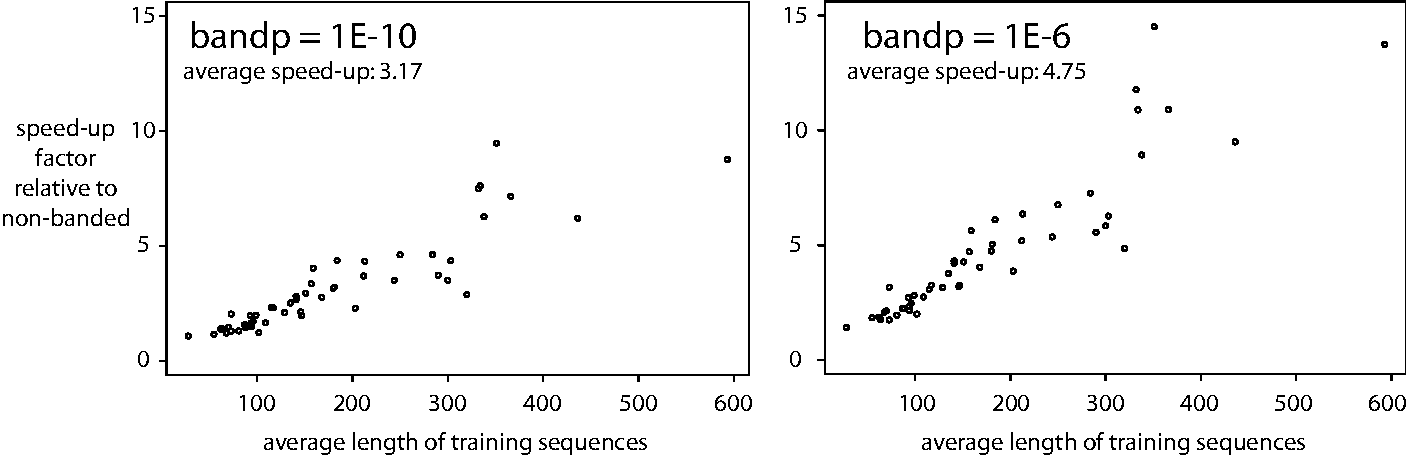
\includegraphics[width=6.4in,angle=0]{figs/scatter}
\caption{\textbf{Acceleration for banded searches of the
    51 benchmark families.} Bands calculated with $bandp =
  10^{-10}$ (probability mass within each band is 99.99999999\%) for
  left plot and $bandp = 10^{-6}$ (probability mass within each band
  is 99.9999\%) for right plot. There are 51 points in each plot, one
  for each family in the benchmark set, representing the speed-up
  for a banded search relative to a non-banded search for the
  corresponding family.}
\label{fig:scatter}
\end{center}
\end{figure}
\fi

\subsection{Benchmark performance}
Acceleration from the banded approach is not useful it comes
at a significant cost to sensitivity. 
To measure the extent of this cost, \emph{summary} MER statistics were
calculated from the master lists of hits to 
describe the performance of a method if a single threshold must
be chosen for all families (and that threshold could be chosen
\emph{after} the results are collected). This score threshold may be
used in future searches, hopefully resulting in similar sensitivity and specificity
measures. Additionally, \emph{family specific} MER statistics were
calculated from the family specific lists of hits, which explain
the performance that could be achieved if different optimal thresholds
were used for each family. Table~\ref{tbl:rmarkmerlist} lists the
summary MER statistic, and family-specific MER statistics (the sum
over all 51 families) for each method tested.
Table~\ref{tbl:rmarkmer_fam} contains the
individual family-specific MER statistics of selected methods.
Figure~\ref{fig:roc} displays the benchmark performance
of the various methods differently, as a ROC plot with sensitivity and
specificity measures for every possible cut point threshold in the
master ranked list of hits (each method from 
Table~\ref{tbl:rmarkmerlist} except for row 3 is included in the
Figure~\ref{fig:roc} ROC plot).


%%%%%%%%%%%%%%%%%%%%%%%%%%%%%%%%%%%%%%%%%%%%%%%%%%%%%%%%%%%%%%%%%%%%%%%
% The rmark MER table - summary MERs
%\normalfont\ttfamily
\ifdraft
\begin{table}[htb]
\begin{center}
%\begin{tabular}{|c|c|ccc|cc|} 
\begin{tabular}{ccccccc} 

%\multicolumn{1}{c}{} & \multicolumn{1}{c}{} & \multicolumn{1}{c}{} &
%\multicolumn{1}{c}{} & \multicolumn{1}{c}{} & \multicolumn{1}{c}{} &
%\multicolumn{1}{c}{summed} \\

\multicolumn{1}{c}{} & \multicolumn{1}{c}{} & \multicolumn{1}{c}{} &
\multicolumn{1}{c}{} & \multicolumn{1}{c}{} &
\multicolumn{1}{c}{summary} & \multicolumn{1}{c}{family-specific} \\

\multicolumn{1}{c}{} & \multicolumn{1}{c}{program} &
\multicolumn{1}{c}{prior} & \multicolumn{1}{c}{entropy (bits)} &
\multicolumn{1}{c}{$bandp$} & \multicolumn{1}{c}{MER} &
\multicolumn{1}{c}{MER} \\ \hline

%1 & \blast-W3 & - & - & - & - & 220 & 189 & 330 & 227 & 376 & 237 \\
1 & \blast & - & - & - & 216 & 188 \\
%3 & \blast-W11 & - & - & - & - & 244 & 218 & 294 & 242 & 341 & 262 \\ \hline
%4 & \infernal glocal & N & - & - & - & 275 & 229 & - & - & - & - \\
%5 & \infernal glocal & Y & - & - & - & 253 & 215 & - & - & - & - \\
%6 & \infernal glocal & Y & 0.54 & - & - & 155 & 104 & 80 & 53 & 69 & 28 \\
%7 & \infernal glocal & Y & 0.54 & - & 1E-6 & 161 & 112 & - & - & - & - \\
%8 & \infernal glocal & Y & 0.54 & - & 1E-10 & 155 & 105 & - & - & - & - \\ \hline
2 & \infernal & plus-1 & - & - & 230 & 184 \\
3 & \infernal & informative & - & - & 188 & 163 \\
%4 & \infernal & Y & 1.46 & - & 122 & 94 \\
4 & \infernal & informative & 1.46 & - & 104 & 90 \\
5 & \infernal & informative & 1.46 & $10^{-6}$ & 116 & 98 \\
6 & \infernal & informative & 1.46 & $10^{-10}$ & 110 & 94 \\ 
\end{tabular}
\end{center}
\caption{\textbf{Rfam benchmark MER summary statistics.} 
    prior: ``plus-1'' if uninformative Laplace plus-1 priors were
    used; ``informative'' if new Dirichlet priors were used.
    entropy: target model entropy in bits for entropy weighting; ``-''
    if entropy weighting was not used.
    %(effective sequence number is number of sequences in training alignment).
    %    EL: EL self transition probability used.
    ``$bandp$'': tail probability loss for banded calculation used; ``-'' if search
    was non-banded. summary MER: MER across 51 benchmark
    families; family-specific MER: MER for each family, summed
    over all 51 families. Program versions: Row 1: WU-BLASTN-2.0MP
    --kap -W=7. Row 2: \infernal version 0.55. Rows 3-6: \infernal
    version 0.70.}
\label{tbl:rmarkmerlist}
\end{table}
\fi

\ifdraft
\begin{figure}
\begin{center}
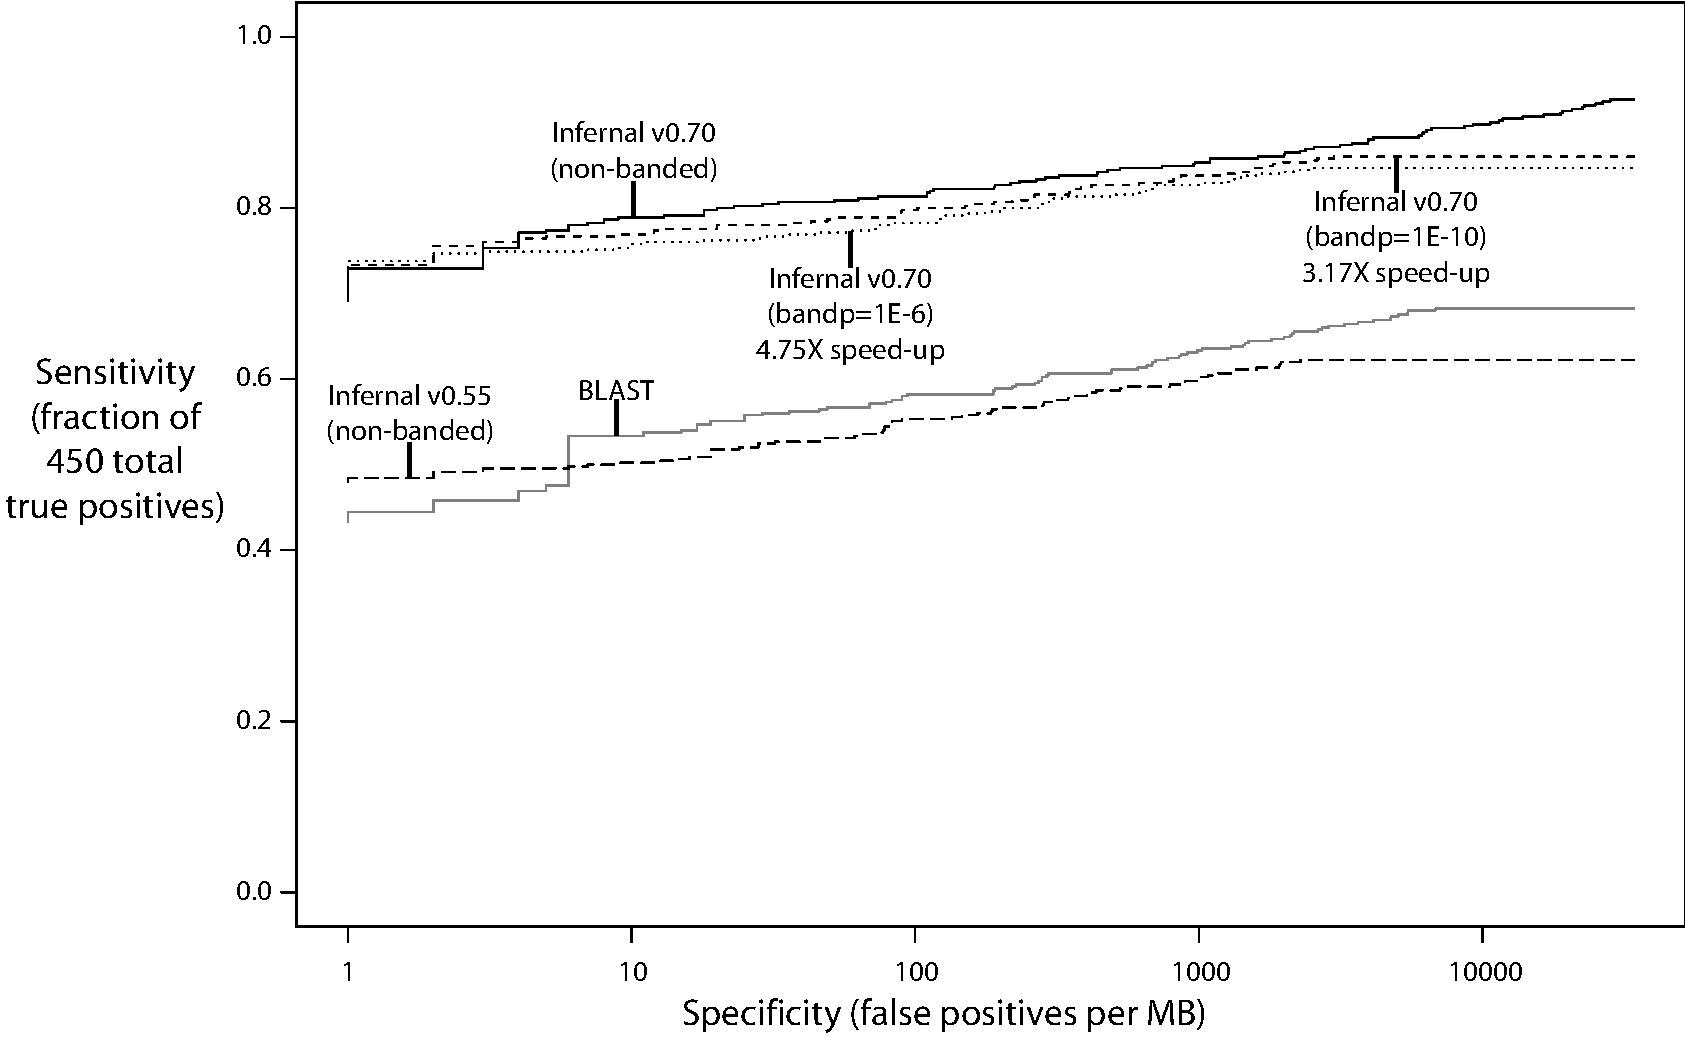
\includegraphics[width=6.4in,angle=0]{figs/d2roc_ai}
\end{center}
\caption{\textbf{ROC curve for the Rfam based benchmark.}  
\blast: corresponds with row 1 of Table~\ref{tbl:rmarkmerlist};
version and options used: \texttt{WU-BLASTN-2.0MP --kap -W=7}. 
\infernal v0.55 (non-banded): corresponds with row 2 of Table~\ref{tbl:rmarkmerlist}.
\infernal v0.70 (non-banded): corresponds with row 4 of Table~\ref{tbl:rmarkmerlist}.
\infernal v0.70 ($bandp=10^{-6}$): corresponds with row 5 of Table~\ref{tbl:rmarkmerlist}.
\infernal v0.70 ($bandp=10^{-10}$): corresponds with row 6 of Table~\ref{tbl:rmarkmerlist}.
 Speed-up statistics for banded runs are averages over the 51 Rfam
 benchmark families.}
\label{fig:roc}
\end{figure}
\fi

\section{Discussion}

The benchmark results summarized in Tables~\ref{tbl:rmarkmerlist} and
\ref{tbl:rmarkmer_fam} and Figures~\ref{fig:scatter} and \ref{fig:roc}
demonstrate the following:

\begin{itemize}
\item
\textbf{The informative priors alone boost performance.}
Incorporating the new priors drops the summary MER from 230 to 188,
and the family specific MER from 184 to 163
(Table~\ref{tbl:rmarkmerlist}, row 2 versus 3). Figure \ref{fig:roc}
demonstrates that the sensitivity increase does not sacrifice specificity.

\item
\textbf{Entropy weighting significantly elevates performance.}
Enforcing a target model entropy brings the summary MER from 188 down to
104, and the family specific MER from 163 down to 90. 
(Table~\ref{tbl:rmarkmerlist}, row 4 versus row 2). Figure~\ref{fig:roc}
demonstrates that the sensitivity increase does not sacrifice
specificity.
 (THIS IS
MISLEADING, THE EL SELF TRANSITION ALSO CHANGES BETWEEN THESE ROWS).

\item
\textbf{The banded strategy offers acceleration with a small cost to
performance.} Using a $bandp$ of $10^{-6}$ results in an average
speed-up per family of 4.75 fold and a total speed-up of 6.74 fold for the
entire benchmark set (Table~\ref{tbl:rmarkmer_fam}).  This speed up
increases summary MER from 104 to 116 and
the family specific MER from 90 to 98 (Table~\ref{tbl:rmarkmerlist},
rows 6 versus row 5). A $bandp$ of $10^{-10}$ gives a smaller
3.17 fold average and 4.40 fold total acceleration
(Table~\ref{tbl:rmarkmer_fam} at a smaller cost to performance;
the summary MER is 110 and the family MER is 94 (row 7 versus row
5). Figure~\ref{fig:roc} is perhaps more informative, showing sensitivity
as a function of specificity.
\end{itemize}

We have presented separate techniques to improve the speed and 
sensitivity of CM based homology search. 
%Our benchmark
%results suggest that the improved sensitivity does not
%sacrifice specificity (Figure~\ref{fig:roc}). However, the speed-up
%from the banded strategy does come at a small cost to sensitivity
%(Figure~\ref{fig:roc}). 
The informative prior distributions are central to both of these
improvements. Informative transitions priors are critical to
the band calculation (Figure~\ref{fig:3bands}), and informative
emission priors allow effective model entropy weighting. Our training
datasets for prior estimation are not ideal: very few counts were used
to estimate many of the transition priors
(Table~\ref{tbl:transitions}), and only ribosomal RNA alignments were
used for to derive counts for the  emission priors. We were driven to
both datasets by a lack of better options. Despite this, the resulting
priors seem to perform well. We hope that the CM methods we have
improved on here will help to provide better training data for future
tools. While we recognize that this approach of building tools using
sparse data to amass better data for use in tool building is circular,
we feel that such an approach is necessary in this case (?).

The model entropy weighting strategy has important implications for
profile HMM filtering methods that rely on primary sequence
conservation.  When building a CM from an input training alignment
with many highly identical sequences, entropy weighting will create a
model with lower information content than a model built using previous
methods (i.e. without entropy weighting). This is because the weight of
the observations from the input alignment will be scaled down
relative to the prior during parameterization.  Profile HMM filters built
from such CMs will also tend to have low information content. In
general, these models will give higher scores (relative to models with
higher information content) to sequences with lowers
sequence identity to the training sequences, making them less
efficient filters. In contrast, entropy weighting will not affect an
initial filtering step by \textsc{BLAST}, as this step is completely
independent of the CM. However, the overall sensitivity of a
\textsc{BLAST} filtering approach may be increased, but only if the
more sensitive entropy weighted CM finds hits in the filtered fraction
that would be missed by CMs built without entropy weighting.

\begin{comment}In contrast, the database fraction that is filtered
by \blast will be unaffected by entropy weighting because it is completely
independent of the CM\@. However, the filtering strategy limits
the CM search to the filtered fraction, so using \textsc{BLAST} as a
filter for entropy weighted CMs will only find 
hits that were found by \textsc{BLAST} and missed by . 

this technique will 
become more sensitive with entropy weighted CMs only by the margin
that \textsc{BLAST} was more sensitive than CMs prior to entropy
weighting (which Figure~\ref{fig:roc} suggests was small).
%so unless \textsc{BLAST} was more sensitive than CMs prior to entropy
%weighting (which Figure~\ref{fig:roc} suggests is unlikely)
%homology., using entropy weighted models will not increase the
%sensitivity of a \textsc{BLAST} filtered CM search. 

However, the \blast strategy still limits
the CM search to only the filtered fraction, which is undesirable
because the sensitivity cost is unknown, and Figure~\ref{fig:roc}
suggests that this cost is likely significant, at least for remote
homology.
\end{comment}

We believe the most important contribution of this work is the
\emph{a priori} banded strategy for accelerating CM homology
search. A filtering approach and the banded strategy are
complementary; the former reduces the search space for the expensive
CM search, and the latter makes CM search less expensive.
\begin{comment}
; i.e.
when performing a search, combining a filtering strategy that
eliminates all but 10\% of the database, and a banded strategy that
speeds up the CM search of the remaining fraction by 10 fold will
employ the CM for only 1\% of the time a non-banded, non-filtered CM
search would have.
\end{comment}
The band calculation method presented here is only one potential
method for determining bands. There are certainly many others. 
The banded CM CYK database algorithm can use bands on subsequence
lengths derived from any method.
However, the band calculation method we present is ideal for homology search in
one important respect. Because the bands are sequence independent and are
determined solely from the transition probabilities of the model, they
can be calculated once, in a few seconds prior to searching, 
adding a relatively negligible amount of time to the overall search.
Other potential banded strategies that consider the sequence (like
Brown's profile HMM based method in \textsc{RNACAD} \cite{Brown00})
need to continuously recalculate the bands as the database is
scanned. Even so, we feel that sequence dependent banding strategies
are promising for accelerating CM methods, and are currently exploring
such techniques.
As complementary filtering and banding methods continue to mature, we
hope CM homology search will become more practical and widespread,
contributing meaningfully to the understanding of non-coding RNAs.

\begin{comment}
currently exploring some ourselves, including methods that do consider
the sequence being searched. As filtering methods and complementary
banded strategies continue to mature, we hope CM homology search
will become more practical and widespread, contributing meaningfully
to the understanding of non-coding RNAs.

Because the bands can be calculated independently of the
database, they only need to be calculated once 
This acceleration technique is
orthogonal to filtering technique accelerates CM
based homology search,  CM
sea

The band calculation algorithm 
offer complements filtering. We speculate
that for many families the speed decrease of a profile HMM based
filtering approach owing to entropy weighting will be completely
offset or surpassed by acceleration from the bands.

for acceleration is 
independent of primary sequence conservation. The speed-up factor is
controlled by the width of the bands, which is itself determined by
the $bandp$ parameter and the transition probabilities of the model,
which are determined by the priors and the 


, and the length
variation in homologous substructures in training sequences of the
family being modelled. Substructure regions that exhibit a lot of
length variation will have permissive transition
probabilities that result in wide bands, and vice versa. Importantly,
the banded strategy complements filtering, 

The sequence independent, \emph{a priori} band calculation strategy
introduced here is only one possible band calculation method. There
are certainly other, potentially more effective, banded strategies. We are
currently exploring some ourselves, including methods that do consider
the sequence being searched. As filtering methods and complementary
banded strategies continue to mature, we hope CM homology search
will become more practical and widespread, contributing meaningfully
to the understanding of non-coding RNAs.

\end{comment}
%%%%%%%%%%%%%%%%%%%%%%%%%%%%%%%%%%%%%%%%%%%%%%%%%%%%%%%%%%%%%%%%%%%%%%%
% The rmark by family MER table
\ifdraft
\renewcommand{\baselinestretch}{1.0}
\begin{table}
%\tiny
\scriptsize
\begin{center}
\begin{tabular}{|ll|rrr|rrrrl|rrrrr|} \hline
\multicolumn{1}{|c}{Rfam 7.0} & \multicolumn{1}{c|}{family} & \multicolumn{1}{c}{\#} & \multicolumn{1}{c}{\#} & \multicolumn{1}{c}{mean len} & \multicolumn{5}{|c|}{\textsc{BLAST}} & \multicolumn{5}{|c|}{\textsc{Infernal}} \\ 
\multicolumn{1}{|c}{ID} & \multicolumn{1}{c|}{name} & \multicolumn{1}{c}{train} & \multicolumn{1}{c}{test} & \multicolumn{1}{c|}{(train)} & \multicolumn{1}{c}{MER} & \multicolumn{1}{c}{TP} & \multicolumn{1}{c}{FP} & \multicolumn{1}{c}{FN} & \multicolumn{1}{c|}{thr} & \multicolumn{1}{c}{MER} & \multicolumn{1}{c}{TP} & \multicolumn{1}{c}{FP} & \multicolumn{1}{c}{FN} & \multicolumn{1}{c|}{thr} \\ \hline 
RF00002 & 5\_8S\_rRNA & 62 & 1 & 151 & 0 & 1 & 0 & 0 & 0.0045 & 0 & 1 & 0 & 0 &  11.27 \\  
RF00003 & U1 & 46 & 6 & 159 & 2 & 4 & 0 & 2 &  0.049 & 0 & 6 & 0 & 0 &  12.26 \\  
RF00004 & U2 & 76 & 1 & 184 & 0 & 1 & 0 & 0 &  0.017 & 0 & 1 & 0 & 0 &     10.00 \\  
RF00005 & tRNA & 1080 & 19 & 73 & 18 & 1 & 0 & 18 &  0.021 & 6 & 13 & 0 & 6 &  14.09 \\  
RF00008 & Hammerhead\_3 & 82 & 1 & 55 & 1 & 0 & 0 & 1 &    0.3 & 0 & 1 & 0 & 0 &   14.70 \\  
RF00009 & RNaseP\_nuc & 26 & 21 & 320 & 19 & 2 & 0 & 19 &   0.02 & 17 & 4 & 0 & 17 &  11.67 \\  
RF00010 & RNaseP\_bact\_a & 233 & 1 & 332 & 0 & 1 & 0 & 0 & 0.00086 & 0 & 1 & 0 & 0 &  12.61 \\  
RF00011 & RNaseP\_bact\_b & 30 & 1 & 366 & 0 & 1 & 0 & 0 &   0.63 & 0 & 1 & 0 & 0 &  12.32 \\  
RF00012 & U3 & 6 & 5 & 212 & 3 & 2 & 0 & 3 &  0.044 & 2 & 3 & 0 & 2 &  16.86 \\  
RF00015 & U4 & 25 & 1 & 141 & 1 & 0 & 0 & 1 &   0.04 & 1 & 0 & 0 & 1 &  13.44 \\  
RF00017 & SRP\_euk\_arch & 28 & 21 & 303 & 19 & 2 & 0 & 19 &   0.52 & 7 & 14 & 0 & 7 &  12.84 \\  
RF00018 & CsrB & 8 & 1 & 351 & 0 & 1 & 0 & 0 &      0.0 & 0 & 1 & 0 & 0 &  12.97 \\  
RF00019 & Y & 15 & 1 & 94 & 1 & 0 & 0 & 1 &  0.073 & 1 & 0 & 0 & 1 &   15.10 \\  
RF00020 & U5 & 29 & 3 & 115 & 1 & 2 & 0 & 1 &  0.054 & 0 & 3 & 0 & 0 &  13.64 \\  
RF00023 & tmRNA & 19 & 40 & 334 & 6 & 34 & 0 & 6 &  0.081 & 9 & 31 & 0 & 9 &  13.14 \\  
RF00024 & Telomerase-vert & 20 & 11 & 436 & 0 & 11 & 0 & 0 &   0.92 & 0 & 11 & 0 & 0 &   11.30 \\  
RF00025 & Telomerase-cil & 10 & 2 & 157 & 2 & 0 & 0 & 2 &  0.005 & 2 & 0 & 0 & 2 &  13.97 \\  
RF00028 & Intron\_gpI & 5 & 24 & 300 & 20 & 4 & 0 & 20 &   0.92 & 13 & 11 & 0 & 13 &  12.25 \\  
RF00029 & Intron\_gpII & 7 & 11 & 141 & 6 & 5 & 0 & 6 &  0.098 & 1 & 10 & 0 & 1 &  11.08 \\  
RF00030 & RNase\_MRP & 18 & 3 & 284 & 3 & 0 & 0 & 3 &  0.003 & 3 & 0 & 0 & 3 &  12.46 \\  
RF00031 & SECIS & 11 & 24 & 64 & 23 & 1 & 0 & 23 &  0.71 & 13 & 13 & 2 & 11 &  14.58 \\  
RF00033 & MicF & 8 & 1 & 93 & 0 & 1 & 0 & 0 &   0.49 & 0 & 1 & 0 & 0 &  13.17 \\  
RF00037 & IRE & 36 & 1 & 28 & 1 & 0 & 0 & 1 &  0.995 & 1 & 0 & 0 & 1 &  14.98 \\  
RF00040 & me5 & 6 & 1 & 338 & 0 & 1 & 0 & 0 &   0.89 & 0 & 1 & 0 & 0 &  11.78 \\  
RF00054 & U25 & 5 & 1 & 87 & 1 & 0 & 0 & 1 &   0.68 & 1 & 0 & 0 & 1 &  16.66 \\  
RF00055 & snoZ37 & 5 & 1 & 94 & 1 & 0 & 0 & 1 &   0.75 & 1 & 0 & 0 & 1 &  13.96 \\  
RF00059 & THI & 228 & 8 & 109 & 2 & 6 & 0 & 2 & 0.0018 & 0 & 8 & 0 & 0 &  13.66 \\  
RF00066 & U7 & 28 & 2 & 62 & 0 & 2 & 0 & 0 &   0.49 & 0 & 2 & 0 & 0 &  14.23 \\  
RF00067 & U15 & 9 & 3 & 146 & 1 & 2 & 0 & 1 &   0.13 & 1 & 2 & 0 & 1 &  22.46 \\  
RF00080 & yypP-ykoY & 20 & 33 & 129 & 29 & 5 & 1 & 28 &   0.11 & 1 & 32 & 0 & 1 &  17.84 \\  
RF00096 & U8 & 5 & 1 & 135 & 0 & 1 & 0 & 0 &  0.024 & 0 & 1 & 0 & 0 &  13.25 \\  
RF00101 & SraC\_RyeA & 6 & 1 & 250 & 0 & 1 & 0 & 0 &    0.2 & 0 & 1 & 0 & 0 &  11.87 \\  
RF00104 & mir-10 & 9 & 2 & 73 & 2 & 0 & 0 & 2 &   0.17 & 2 & 0 & 0 & 2 &  16.13 \\  
RF00114 & S15 & 10 & 1 & 117 & 1 & 0 & 0 & 1 &  0.029 & 1 & 0 & 0 & 1 &  16.94 \\  
RF00163 & Hammerhead\_1 & 65 & 1 & 68 & 1 & 0 & 0 & 1 &   0.36 & 0 & 1 & 0 & 0 &  16.52 \\  
RF00165 & Corona\_pk3 & 10 & 1 & 63 & 1 & 0 & 0 & 1 &   0.82 & 1 & 0 & 0 & 1 &  14.72 \\  
RF00167 & Purine & 33 & 4 & 99 & 0 & 4 & 0 & 0 &   0.13 & 0 & 4 & 0 & 0 &  13.02 \\  
RF00168 & Lysine & 33 & 17 & 180 & 4 & 13 & 0 & 4 &  0.036 & 0 & 17 & 0 & 0 &  15.98 \\  
RF00169 & SRP\_bact & 46 & 15 & 96 & 3 & 12 & 0 & 3 &   0.08 & 0 & 15 & 0 & 0 &  14.22 \\  
RF00170 & msr & 5 & 3 & 70 & 3 & 0 & 0 & 3 &   0.49 & 3 & 0 & 0 & 3 &  13.49 \\  
RF00174 & Cobalamin & 87 & 66 & 203 & 0 & 66 & 0 & 0 &  0.021 & 0 & 66 & 0 & 0 &   15.90 \\  
RF00177 & SSU\_rRNA\_5 & 145 & 21 & 593 & 3 & 19 & 1 & 2 &   0.58 & 0 & 21 & 0 & 0 &   9.89 \\  
RF00206 & U54 & 12 & 1 & 81 & 1 & 0 & 0 & 1 &  0.054 & 1 & 0 & 0 & 1 &   15.80 \\  
RF00213 & snoR38 & 7 & 3 & 88 & 1 & 2 & 0 & 1 &   0.49 & 0 & 3 & 0 & 0 &  16.07 \\  
RF00230 & T-box & 10 & 35 & 244 & 4 & 31 & 0 & 4 & 0.9992 & 1 & 34 & 0 & 1 &  12.34 \\  
RF00234 & glmS & 8 & 3 & 181 & 0 & 3 & 0 & 0 &   0.16 & 0 & 3 & 0 & 0 &  11.88 \\  
RF00373 & RNaseP\_arch & 20 & 13 & 290 & 1 & 12 & 0 & 1 &  0.003 & 0 & 13 & 0 & 0 &  19.39 \\  
RF00379 & ydaO-yuaA & 31 & 4 & 147 & 0 & 4 & 0 & 0 &  0.026 & 0 & 4 & 0 & 0 &  13.11 \\  
RF00380 & ykoK & 35 & 3 & 168 & 0 & 3 & 0 & 0 &  0.073 & 0 & 3 & 0 & 0 &  13.13 \\  
RF00448 & IRES\_EBNA & 7 & 1 & 213 & 0 & 1 & 0 & 0 &   0.79 & 1 & 0 & 0 & 1 &  11.99 \\  
RF00504 & gcvT & 109 & 5 & 102 & 3 & 2 & 0 & 3 &   0.04 & 0 & 5 & 0 & 0 &   13.40 \\ \hline 
%\multicolumn{2}{c}{summed family} & 56 & 8 & ? & 188 & 264 & 2 & 186 &  0.017 & 90 & 362 & 2 & 88 &  16.38 \\  
%\multicolumn{15}{c}{} \\ \hline
\multicolumn{5}{|c|}{MER statistics summed across all families} & 188
& 264 & 2 & 186 & N/A & 90 & 362 & 2 & 88 & N/A \\  
\multicolumn{5}{|c|}{Summary MER statistics (using one threshold for
all families)} & 216 & 240 & 6 & 210 &  0.017 & 104 & 354 & 8 & 96 &  16.38 \\ \hline 
%total(fam) & & 56 & 8 & ? & 188 & 264 & 2 & 186 &  0.017 & 90 & 362 & 2 & 88 &  16.38 \\  
%total & & 2874 & 450 & ? & 216 & 240 & 6 & 210 &  0.017 & 104 & 354 & 8 & 96 &  16.38 \\  
\end{tabular}
\end{center}

\caption{\textbf{Rfam benchmark families with MER statistics.}
  The minimum error rate (MER) threshold is the score for a given
  method searching for a given Rfam family at which the sum of false
  positives (FP) and false negatives (FN) is
  minimized. ``MER''= FP+FN at threshold. ``TP''= TP at
  threshold. ``thr''= threshold; E-value (\textsc{BLAST}) or bit score
  (\textsc{Infernal}). For the row labelled
  ``Summary MER statistics'': MER statistics are derived from ranked list
  of all hits across all families. ``mean len (train)'' = mean length
  of training sequences in benchmark set. 
  Program versions and options used: \textsc{BLAST}=
  WU-BLASTN-2.0MP --kap -W=7. \textsc{Infernal}= cmsearch
  --local (version 0.70)}

\label{tbl:rmarkmer_fam}
\end{table}
\fi

% The rmark local speed up table
\ifdraft
\begin{table}
\scriptsize
\begin{center}
\begin{tabular}{|ll|rrr|rr|rr|r|} \cline{6-10}
\multicolumn{5}{c}{} & \multicolumn{2}{|c|}{$bandp = 10^{-10}$} &
  \multicolumn{2}{c|}{$bandp = 10^{-6}$} & \multicolumn{1}{c|}{non-banded} \\ \cline{1-5}
Rfam ID & family & avg len & W & bifs & time & spd up & time & spd up & time \\ \hline 
RF00177 & SSU\_rRNA\_5 & 593 & 791 & 12 & 17.36 & 8.76 & 11.07 & 13.74 & 152.08 \\  
RF00024 & Telomerase-vert & 436 & 757 & 2 & 10.33 & 6.21 & 6.75 & 9.50 & 64.09 \\  
RF00011 & RNaseP\_bact\_b & 366 & 638 & 9 & 8.76 & 7.16 & 5.75 & 10.91 & 62.69 \\  
RF00018 & CsrB & 351 & 439 & 10 & 5.32 & 9.47 & 3.47 & 14.51 & 50.37 \\  
RF00040 & rne5 & 338 & 369 & 4 & 5.88 & 6.27 & 4.13 & 8.93 & 36.88 \\  
RF00023 & tmRNA & 334 & 648 & 4 & 5.70 & 7.63 & 3.99 & 10.89 & 43.46 \\  
RF00010 & RNaseP\_bact\_a & 332 & 881 & 7 & 7.94 & 7.49 & 5.06 & 11.77 & 59.52 \\  
RF00009 & RNaseP\_nuc & 320 & 709 & 4 & 18.13 & 2.89 & 10.78 & 4.86 & 52.40 \\  
RF00017 & SRP\_euk\_arch & 303 & 339 & 3 & 6.26 & 4.37 & 4.36 & 6.27 & 27.34 \\  
RF00028 & Intron\_gpI & 300 & 460 & 4 & 8.98 & 3.51 & 5.40 & 5.85 & 31.55 \\  
RF00373 & RNaseP\_arch & 290 & 439 & 4 & 7.39 & 3.73 & 4.96 & 5.57 & 27.58 \\  
RF00030 & RNase\_MRP & 284 & 460 & 5 & 7.65 & 4.62 & 4.86 & 7.27 & 35.36 \\  
RF00101 & SraC\_RyeA & 250 & 276 & 4 & 3.73 & 4.62 & 2.54 & 6.76 & 17.20 \\  
RF00230 & T-box & 244 & 338 & 1 & 4.37 & 3.51 & 2.86 & 5.36 & 15.32 \\  
RF00448 & IRES\_EBNA & 213 & 246 & 4 & 2.90 & 4.34 & 1.98 & 6.36 & 12.57 \\  
RF00012 & U3 & 212 & 236 & 2 & 3.56 & 3.70 & 2.53 & 5.20 & 13.16 \\  
RF00174 & Cobalamin & 203 & 458 & 3 & 7.33 & 2.29 & 4.34 & 3.87 & 16.81 \\  
RF00004 & U2 & 184 & 219 & 4 & 2.45 & 4.37 & 1.75 & 6.11 & 10.72 \\  
RF00234 & glmS & 181 & 434 & 3 & 4.48 & 3.21 & 2.85 & 5.04 & 14.36 \\  
RF00168 & Lysine & 180 & 277 & 3 & 3.32 & 3.16 & 2.22 & 4.74 & 10.51 \\  
RF00380 & ykoK & 168 & 208 & 2 & 2.83 & 2.77 & 1.94 & 4.05 & 7.85 \\  
RF00003 & U1 & 159 & 184 & 3 & 1.93 & 4.04 & 1.38 & 5.64 & 7.78 \\  
RF00025 & Telomerase-cil & 157 & 202 & 2 & 2.21 & 3.37 & 1.58 & 4.72 & 7.44 \\  
RF00002 & 5\_8S\_rRNA & 151 & 224 & 2 & 2.22 & 2.95 & 1.53 & 4.28 & 6.54 \\  
RF00379 & ydaO-yuaA & 147 & 317 & 3 & 4.09 & 1.97 & 2.48 & 3.26 & 8.07 \\  
RF00067 & U15 & 146 & 187 & 0 & 2.31 & 2.13 & 1.54 & 3.20 & 4.92 \\  
RF00015 & U4 & 141 & 289 & 3 & 2.39 & 2.81 & 1.56 & 4.32 & 6.72 \\  
RF00029 & Intron\_gpII & 141 & 286 & 1 & 3.23 & 2.67 & 2.05 & 4.21 & 8.62 \\  
RF00096 & U8 & 135 & 198 & 2 & 2.14 & 2.52 & 1.43 & 3.77 & 5.38 \\  
RF00080 & yybP-ykoY & 129 & 287 & 2 & 2.62 & 2.11 & 1.75 & 3.16 & 5.53 \\  
RF00114 & S15 & 117 & 138 & 1 & 1.41 & 2.31 & 1.00 & 3.26 & 3.26 \\  
RF00020 & U5 & 115 & 141 & 1 & 1.57 & 2.32 & 1.18 & 3.08 & 3.63 \\  
RF00059 & THI & 109 & 305 & 2 & 3.68 & 1.67 & 2.23 & 2.75 & 6.14 \\  
RF00504 & gcvT & 102 & 298 & 1 & 3.48 & 1.23 & 2.14 & 2.01 & 4.30 \\  
RF00167 & Purine & 99 & 114 & 1 & 1.30 & 1.99 & 0.92 & 2.82 & 2.60 \\  
RF00169 & SRP\_bact & 96 & 117 & 0 & 1.49 & 1.72 & 1.04 & 2.46 & 2.57 \\  
RF00019 & Y & 94 & 142 & 0 & 1.66 & 1.50 & 1.16 & 2.16 & 2.49 \\  
RF00055 & snoZ37 & 94 & 117 & 0 & 1.21 & 1.65 & 0.86 & 2.33 & 1.99 \\  
RF00033 & MicF & 93 & 126 & 1 & 1.13 & 1.98 & 0.82 & 2.71 & 2.23 \\  
RF00213 & snoR38 & 88 & 169 & 0 & 1.68 & 1.46 & 1.09 & 2.24 & 2.45 \\  
RF00054 & U25 & 87 & 107 & 0 & 1.05 & 1.58 & 0.74 & 2.25 & 1.66 \\  
RF00206 & U54 & 81 & 135 & 0 & 1.24 & 1.31 & 0.83 & 1.96 & 1.62 \\  
RF00005 & tRNA & 73 & 186 & 2 & 1.12 & 2.04 & 0.72 & 3.17 & 2.29 \\  
RF00104 & mir-10 & 73 & 100 & 0 & 1.16 & 1.31 & 0.86 & 1.75 & 1.51 \\  
RF00170 & msr & 70 & 135 & 0 & 1.03 & 1.48 & 0.71 & 2.15 & 1.52 \\  
RF00163 & Hammerhead\_1 & 68 & 238 & 1 & 2.33 & 1.21 & 1.34 & 2.10 & 2.82 \\  
RF00031 & SECIS & 64 & 97 & 0 & 0.90 & 1.37 & 0.70 & 1.76 & 1.24 \\  
RF00165 & Corona\_pk3 & 63 & 78 & 0 & 0.68 & 1.43 & 0.52 & 1.85 & 0.97 \\  
RF00066 & U7 & 62 & 96 & 0 & 0.74 & 1.39 & 0.55 & 1.87 & 1.03 \\  
RF00008 & Hammerhead\_3 & 55 & 164 & 1 & 1.07 & 1.16 & 0.67 & 1.85 & 1.24 \\  
RF00037 & IRE & 28 & 41 & 0 & 0.28 & 1.09 & 0.21 & 1.42 & 0.30 \\ \hline 
\multicolumn{5}{|c|}{average} & 3.88 & 3.17 & 2.53 & 4.75 & 17.07 \\ 
\multicolumn{5}{|c|}{total}   & 198.02 & 4.40 & 129.18 & 6.74 & 870.68 \\ \hline 
\end{tabular}
\end{center}

\caption{\textbf{Statistics and running times for
      \textsc{Infernal} version 0.70 CMs on the Rfam benchmark.} ``bifs''=
      number of bifurcations in consensus secondary
      structure. ``time'': hours per MB. ``spd up'': speed-up factor
      relative to non-banded. All searches performed in local mode.}
\label{tbl:rmarkbtimes_l}
\end{table}
\fi

\section{Acknowledgements}
EPN gratefully acknowledges financial support from NIH training grant
X. 

\newpage
%\bibliography{distilled}
\bibliography{master,books,lab,bandcyk}

\ifdraft
 \relax
\else
\newpage
\begin{figure}
\begin{center}
\caption{\textbf{A simplified CM.} \textbf{(A):} Biologically
  unrealistic, toy CM with simplified architecture. \textbf{(B):} Examples of
  sequences generated from CM in (A), each with its own probability
  given the transition probabilities of the model, as shown in plots at
   bottom.}
\label{fig:aprioriAB}
\end{center}
\end{figure}

\begin{figure}
\begin{center}
\caption{\textbf{A trace of the band calculation
  algorithm for the simplified CM in Figure~\ref{fig:aprioriAB}.} 
    The maximum length $d$ considered (the $Z$ parameter) is set as
    10. Resulting $\gamma$ probability distributions shown at right. For
    state $0$ (step 7), the $\gamma$ plot is color-coded to correspond
    with probabilities in Figure~\ref{fig:aprioriAB}.}
\label{fig:aprioriC}
\end{center}
\end{figure}

\begin{figure}
  \begin{center}
    \label{fig:3bands}
    \caption{\textbf{Effect of transition priors on band calculation.}
  Solid vertical lines represent the lengths of the 5
  seed sequences used to build each model, corresponding with the
  right vertical axis labels. Band calculation is compared using
  ``plus-1'' transition priors and the newly estimated ``informative''
  Dirichlet priors as follows: Dashed
  probability distributions show $\gamma_0(d)$, the probability a
  sequence of length $d$ is generated by state $0$ (the top-most, root state)
  of each model. Dashed vertical lines are the band ($dmin_0$ (left) and
  $dmax_0$ (right)) derived from the $\gamma_0(d)$ distribution using $bandp =
  10^{-7}$ (probability mass within each band is 99.99999\%).}
  \end{center}
\end{figure}

\renewcommand{\baselinestretch}{1.0}
\begin{table}
\renewcommand{\tabcolsep}{0.7em}
\tiny
\begin{center}
%\begin{tabular}{|r|r|l|l|l||l|r||l|r||l|r||l|r||l|r||l|r||} \hline
\begin{tabular}{|rr|rr|cc|c|c|cc|cc|cc|cc|cc|cc|} \cline{1-6} \cline{8-20}
%\multicolumn{5}{c}{} & \multicolumn{2}{|c|}{1} & \multicolumn{2}{|c|}{2} & \multicolumn{2}{|c|}{3} & \multicolumn{2}{|c|}{4} & \multicolumn{2}{|c|}{5} & \multicolumn{2}{|c|}{6} \\ \cline{1-17}
\multicolumn{1}{|c}{alph} & \multicolumn{1}{c|}{grp} &
  \multicolumn{1}{c}{alph} & \multicolumn{1}{c|}{grp} & node & next &
  & \multicolumn{13}{|c|}{transition alphabets and Dirichlet $\alpha$ parameters} \\ %\cline{8-20}
%\multicolumn{1}{|c}{\#} & \multicolumn{1}{c|}{\#} & \multicolumn{1}{c}{counts} & \multicolumn{1}{c|}{counts} & state & node & & $|\alpha|$ & $a_1$ &
%  $\frac{\alpha_{a_1}}{|\alpha|}$ & $a_2$ & $\frac{\alpha_{a_2}}{|\alpha|}$ & $a_3$ &
%  $\frac{\alpha_{a_3}}{|\alpha|}$ & $a_4$ & $\frac{\alpha_{a_4}}{|\alpha|}$ & $a_5$ &
%  $\frac{\alpha_{a_5}}{|\alpha|}$ & $a_6$ & $\frac{\alpha_{a_6}}{|\alpha|}$ \\
%  \cline{1-6} \cline {8-20} 
\multicolumn{1}{|c}{\#} & \multicolumn{1}{c|}{\#} & \multicolumn{1}{c}{counts} & \multicolumn{1}{c|}{counts} & state & node & & $|\alpha|$ & $a$ &
  $\frac{\alpha_{a}}{|\alpha|}$ & $a$ & $\frac{\alpha_{a}}{|\alpha|}$ & $a$ &
  $\frac{\alpha_{a}}{|\alpha|}$ & $a$ & $\frac{\alpha_{a}}{|\alpha|}$ & $a$ &
  $\frac{\alpha_{a}}{|\alpha|}$ & $a$ & $\frac{\alpha_{a}}{|\alpha|}$ \\
  \cline{1-6} \cline {8-20} 

1   &    & 6     & 11    & MATP\_MP & BIF  & & 0.5509  & IL & 0.1229 & IR & 0.0001 & B  & 0.8770 &    &        &    &  &  &  \\  
2   &    & 7023  & 7119  & MATP\_MP & MATP & & 7.2986  & IL & 0.0023 & IR & 0.0024 & MP & 0.9816 & ML & 0.0056 & MR & 0.0046 & D & 0.0035 \\  
3   &    & 1600  & 1830  & MATP\_MP & MATL & & 1.5914  & IL & 0.0179 & IR & 0.0155 & ML & 0.9200 & D  & 0.0466 &    &  &  &  \\  
4   &    & 145   & 195   & MATP\_MP & MATR & & 1.9038  & IL & 0.0173 & IR & 0.0073 & MR & 0.8903 & D  & 0.0852 &    &  &  &  \\  
5   & 1  & 2     & 11    & MATP\_MP & END  & & 0.5509  & IL & 0.1229 & IR & 0.0001 & E  & 0.8770 &    &        &    &  &  &  \\  
6*  &    & 1     & 2     & MATP\_ML & BIF  & & 3.0000  & IL & 0.3333 & IR & 0.3333 & B  & 0.3333 &    &        &    &  &  &  \\  
7   &    & 577   & 577   & MATP\_ML & MATP & & 0.6941  & IL & 0.0131 & IR & 0.0103 & MP & 0.4032 & ML & 0.4983 & MR & 0.0115 & D & 0.0636 \\  
8   &    & 133   & 133   & MATP\_ML & MATL & & 0.9316  & IL & 0.0739 & IR & 0.0651 & ML & 0.7038 & D  & 0.1571 &    &  &  &  \\  
9   &    & 15    & 15    & MATP\_ML & MATR & & 0.3272  & IL & 0.1884 & IR & 0.0432 & MR & 0.4082 & D  & 0.3602 &    &  &  &  \\  
10* & 6  & 1     & 2     & MATP\_ML & END  & & 3.0000  & IL & 0.3333 & IR & 0.3333 & E  & 0.3333 &    &        &    &  &  &  \\  
11* &    & 1     & 2     & MATP\_MR & BIF  & & 3.0000  & IL & 0.3333 & IR & 0.3333 & B  & 0.3333 &    &        &    &  &  &  \\  
12  &    & 531   & 531   & MATP\_MR & MATP & & 0.7987  & IL & 0.0079 & IR & 0.0190 & MP & 0.3241 & ML & 0.0193 & MR & 0.5631 & D & 0.0666 \\  
13  &    & 151   & 151   & MATP\_MR & MATL & & 0.6933  & IL & 0.0357 & IR & 0.0699 & ML & 0.3066 & D  & 0.5879 &    &  &  &  \\  
14  &    & 15    & 15    & MATP\_MR & MATR & & 0.3574  & IL & 0.0582 & IR & 0.0002 & MR & 0.7629 & D  & 0.1787 &    &  &  &  \\  
15* & 11 & 1     & 2     & MATP\_MR & END  & & 3.0000  & IL & 0.3333 & IR & 0.3333 & E  & 0.3333 &    &        &    &  &  &  \\  
16* &    & 0     & 2     & MATP\_D  & BIF  & & 3.0000  & IL & 0.3333 & IR & 0.3333 & B  & 0.3333 &    &        &    &  &  &  \\  
17  &    & 575   & 575   & MATP\_D  & MATP & & 0.5450  & IL & 0.0019 & IR & 0.0047 & MP & 0.0857 & ML & 0.0534 & MR & 0.0528 & D & 0.8015 \\  
18  &    & 149   & 149   & MATP\_D  & MATL & & 0.5831  & IL & 0.0421 & IR & 0.0526 & ML & 0.2080 & D  & 0.6973 &    &  &  &  \\  
19  &    & 14    & 14    & MATP\_D  & MATR & & 0.1164  & IL & 0.0001 & IR & 0.0001 & MR & 0.2439 & D  & 0.7559 &    &  &  &  \\  
20* & 16 & 2     & 2     & MATP\_D  & END  & & 3.0000  & IL & 0.3333 & IR & 0.3333 & E  & 0.3333 &    &        &    &  &  &  \\  
21  &    & 2     & 4     & MATP\_IL & BIF  & & 1.4397  & IL & 0.6553 & IR & 0.0445 & B  & 0.3002 &    &        &    &  &  &  \\  
22  &    & 121   & 126   & MATP\_IL & MATP & & 0.9402  & IL & 0.1673 & IR & 0.1394 & MP & 0.5904 & ML & 0.0443 & MR & 0.0259 & D & 0.0327 \\  
23  &    & 114   & 119   & MATP\_IL & MATL & & 0.8046  & IL & 0.3108 & IR & 0.1936 & ML & 0.4610 & D  & 0.0346 &    &  &  &  \\  
24  &    & 14    & 15    & MATP\_IL & MATR & & 1.0926  & IL & 0.1419 & IR & 0.0501 & MR & 0.6538 & D  & 0.1541 &    &  &  &  \\  
25  & 21 & 2     & 4     & MATP\_IL & END  & & 1.4397  & IL & 0.6553 & IR & 0.0445 & E  & 0.3002 &    &        &    &  &  &  \\  
26  &    & 1     & 31    & MATP\_IR & BIF  & & 0.9361  & IR & 0.2827 & B  & 0.7173 &    &        &    &        &    &  &  &  \\  
27  &    & 145   & 227   & MATP\_IR & MATP & & 1.5494  & IR & 0.1884 & MP & 0.7090 & ML & 0.0165 & MR & 0.0588 & D  & 0.0273 &  &  \\  
28  &    & 129   & 701   & MATP\_IR & MATL & & 1.6332  & IR & 0.3681 & ML & 0.5752 & D  & 0.0566 &    &        &    &  &  &  \\  
29  &    & 8     & 160   & MATP\_IR & MATR & & 1.2428  & IR & 0.2633 & MR & 0.6809 & D  & 0.0558 &    &        &    &  &  &  \\  
30  & 26 & 0     & 31    & MATP\_IR & END  & & 0.9361  & IR & 0.2827 & E  & 0.7173 &    &        &    &        &    &  &  &  \\  
31  &    & 108   & 1130  & MATL\_ML & BIF  & & 1.2298  & IL & 0.0078 & B  & 0.9922 &    &        &    &        &    &  &  &  \\  
32  &    & 420   & 1319  & MATL\_ML & MATP & & 2.4162  & IL & 0.0132 & MP & 0.9520 & ML & 0.0150 & MR & 0.0129 & D  & 0.0070 &  &  \\  
33  &    & 19013 & 19371 & MATL\_ML & MATL & & 1.8632  & IL & 0.0082 & ML & 0.9711 & D  & 0.0207 &    &        &    &  &  &  \\  
34  &    & 859   & 6692  & MATL\_ML & MATR & & 72.1283 & IL & 0.0058 & MR & 0.9755 & D  & 0.0187 &    &        &    &  &  &  \\  
35  & 31 & 801   & 1130  & MATL\_ML & END  & & 1.2298  & IL & 0.0078 & E  & 0.9922 &    &        &    &        &    &  &  &  \\  
36  &    & 28    & 172   & MATL\_D  & BIF  & & 6.8008  & IL & 0.0029 & B  & 0.9971 &    &        &    &        &    &  &  &  \\  
37  &    & 103   & 103   & MATL\_D  & MATP & & 0.7288  & IL & 0.0321 & MP & 0.5730 & ML & 0.0536 & MR & 0.1654 & D  & 0.1758 &  &  \\  
38  &    & 3152  & 3152  & MATL\_D  & MATL & & 0.4101  & IL & 0.0138 & ML & 0.3105 & D  & 0.6756 &    &        &    &  &  &  \\  
39  &    & 154   & 154   & MATL\_D  & MATR & & 0.6736  & IL & 0.0203 & MR & 0.6014 & D  & 0.3782 &    &        &    &  &  &  \\  
40  & 36 & 144   & 172   & MATL\_D  & END  & & 6.8008  & IL & 0.0029 & E  & 0.9971 &    &        &    &        &    &  &  &  \\  
41  & 26 & 13    & 31    & MATL\_IL & BIF  & & 0.9361  & IL & 0.2827 & B  & 0.7173 &    &        &    &        &    &  &  &  \\  
42  & 27 & 35    & 227   & MATL\_IL & MATP & & 1.5494  & IL & 0.1884 & MP & 0.7090 & ML & 0.0588 & MR & 0.0165 & D  & 0.0273 &  &  \\  
43  & 28 & 549   & 701   & MATL\_IL & MATL & & 1.6332  & IL & 0.3681 & ML & 0.5752 & D  & 0.0566 &    &        &    &  &  &  \\  
44  & 29 & 45    & 160   & MATL\_IL & MATR & & 1.2428  & IL & 0.2633 & MR & 0.6809 & D  & 0.0558 &    &        &    &  &  &  \\  
45  & 26 & 0     & 31    & MATL\_IL & END  & & 0.9361  & IL & 0.2827 & E  & 0.7173 &    &        &    &        &    &  &  &  \\  
46  & 31 & 206   & 1130  & MATR\_MR & BIF  & & 1.2298  & IR & 0.0078 & B  & 0.9922 &    &        &    &        &    &  &  &  \\  
47  & 32 & 848   & 1319  & MATR\_MR & MATP & & 2.4162  & IR & 0.0132 & MP & 0.9520 & ML & 0.0150 & MR & 0.0129 & D  & 0.0070 &  &  \\  
48  & 34 & 5833  & 6692  & MATR\_MR & MATR & & 2.1283  & IR & 0.0058 & MR & 0.9755 & D  & 0.0187 &    &        &    &  &  &  \\  
49  &    & 39    & 39    & MATR\_D  & BIF  & & 0.4664  & IR & 0.0463 & B  & 0.9537 &    &        &    &        &    &  &  &  \\  
50  &    & 176   & 176   & MATR\_D  & MATP & & 0.8689  & IR & 0.0245 & MP & 0.6126 & ML & 0.1269 & MR & 0.0471 & D  & 0.1890 &  &  \\  
51  &    & 771   & 771   & MATR\_D  & MATR & & 0.4869  & IR & 0.0119 & MR & 0.3373 & D  & 0.6507 &    &        &    &  &  &  \\  
52  & 26 & 15    & 31    & MATR\_IR & BIF  & & 0.9361  & IR & 0.2827 & B  & 0.7173 &    &        &    &        &    &   &  &  \\  
53  & 27 & 39    & 227   & MATR\_IR & MATP & & 1.5494  & IR & 0.1884 & MP & 0.7090 & ML & 0.0165 & MR & 0.0588 & D  & 0.0273 &  &  \\  
54  & 29 & 107   & 160   & MATR\_IR & MATR & & 1.2428  & IR & 0.2633 & MR & 0.6809 & D  & 0.0558 &    &        &    &  &  &  \\  
%55 &    &       &       & BEGL\_S  & BIF  & & 1.0000  & B  & 1.0000 &    &        &    &        &    &        &    &  &  &  \\  
55  &    & 338   & 338   & BEGL\_S  & MATP & & 5.0422  & MP & 0.9579 & ML & 0.0121 & MR & 0.0183 & D  & 0.0117 &    &   &  &  \\  
56  & 31 & 15    & 1130  & BEGR\_S  & BIF  & & 1.2298  & IL & 0.0078 & B  & 0.9922 &    &        &    &        &    &  &  &  \\  
57  & 32 & 51    & 1319  & BEGR\_S  & MATP & & 2.4162  & IL & 0.0132 & MP & 0.9520 & ML & 0.0150 & MR & 0.0129 & D  & 0.0070 &  &  \\  
58  & 33 & 358   & 19371 & BEGR\_S  & MATL & & 1.8632  & IL & 0.0082 & ML & 0.9711 & D  & 0.0207 &    &        &    &  &  &  \\  
59  & 26 & 2     & 31    & BEGR\_IL & BIF  & & 0.9361  & IL & 0.2827 & B  & 0.7173 &    &        &    &        &    &   &  &  \\  
60  & 27 & 3     & 227   & BEGR\_IL & MATP & & 1.5494  & IL & 0.1884 & MP & 0.7090 & ML & 0.0588 & MR & 0.0165 & D  & 0.0273 &  &  \\  
61  & 28 & 19    & 701   & BEGR\_IL & MATL & & 1.6332  & IL & 0.3681 & ML & 0.5752 & D  & 0.0566 &    &        &    &  &  &  \\  
62  & 1  & 3     & 11    & ROOT\_S  & BIF  & & 0.5509  & IL & 0.1229 & IR & 0.0001 & B  & 0.8770 &    &        &    &  &  &  \\  
63  & 2  & 96    & 7119  & ROOT\_S  & MATP & & 7.2986  & IL & 0.0023 & IR & 0.0024 & MP & 0.9816 & ML & 0.0056 & MR & 0.0046 & D & 0.0035 \\  
64  & 3  & 230   & 1830  & ROOT\_S  & MATL & & 1.5914  & IL & 0.0179 & IR & 0.0155 & ML & 0.9200 & D  & 0.0466 &    &  &  &  \\  
65  & 4  & 50    & 195   & ROOT\_S  & MATR & & 1.9038  & IL & 0.0173 & IR & 0.0073 & MR & 0.8903 & D  & 0.0852 &    &  &  &  \\  
66  & 21 & 0     & 4     & ROOT\_IL & BIF  & & 1.4397  & IL & 0.6553 & IR & 0.0445 & B  & 0.3002 &    &        &    &  &  &  \\  
67  & 22 & 5     & 126   & ROOT\_IL & MATP & & 0.9402  & IL & 0.1673 & IR & 0.1394 & MP & 0.5904 & ML & 0.0443 & MR & 0.0259 & D & 0.0327 \\  
68  & 23 & 5     & 119   & ROOT\_IL & MATL & & 0.8046  & IL & 0.3108 & IR & 0.1936 & ML & 0.4610 & D  & 0.0346 &    &  &  &  \\  
69  & 24 & 1     & 15    & ROOT\_IL & MATR & & 1.0926  & IL & 0.1419 & IR & 0.0501 & MR & 0.6538 & D  & 0.1541 &    &  &  &  \\  
70  & 26 & 0     & 31    & ROOT\_IR & BIF  & & 0.9361  & IR & 0.2827 & B  & 0.7173 &    &        &    &        &    &  &  &  \\  
71  & 27 & 5     & 227   & ROOT\_IR & MATP & & 1.5494  & IR & 0.1884 & MP & 0.7090 & ML & 0.0165 & MR & 0.0588 & D  & 0.0273 &  &  \\  
72  & 28 & 4     & 701   & ROOT\_IR & MATL & & 1.6332  & IR & 0.3681 & ML & 0.5752 & D  & 0.0566 &    &        &    &  &  &  \\  
73  & 29 & 0     & 160   & ROOT\_IR & MATR & & 1.2428  & IR & 0.2633 & MR & 0.6809 & D  & 0.0558 &    &        &    &  &  &  \\   \cline{1-6} \cline {8-20} 
\end{tabular}
\end{center}
\normalfont\rmfamily
\caption{\textbf{Transition alphabets and groups with corresponding
    training counts and estimated Dirichlet transition prior parameters.}
  ``alph \#''= transition alphabet number; ``*'' indicates a plus-1
  prior is used. ``grp \#''= transition
  group number, each group is numbered as the lowest numbered alphabet in
  group, this column is blank if alphabet number = group
  number. ``alph counts''= observed Rfam 6.1 counts for
  alphabet. ``grp counts''= total Rfam 6.1 counts for group, used
  to estimate Dirichlet prior. ``node state''= initial node state type for each
  alphabet. ``next node''= type of immediately downstream
  node for each alphabet.}
\label{tbl:transitions}
\end{table}
\renewcommand{\baselinestretch}{1.5}

\begin{table}
%\normalfont\ttfamily
\begin{center}
\begin{tabular}{lrrrrrrr} 
& & \# aln & \# filtered & \# consensus & \# consensus & bp & SS \\
alignment & \# seq & columns & seq & bp & SS columns & counts & counts \\ \hline
LSU & 1551 & 7270 & 139 & 601 & 1532 & 65229 & 180558  \\
SSU bap & 12773 & 2653 & 254 & 421 & 680 & 97834 & 153565 \\
SSU euk & 7151 & 4558 & 207 & 407 & 959 & 72521 & 174260 \\
SSU mito & 1039 & 3791 & 107 & 216 & 524 & 19803 & 56510 \\ 
%\multicolumn{8}{l}{bap: contains bacterial, archaeal and plastid
%  sequences} \\
\end{tabular}
\caption{\textbf{Statistics on the alignments used for emission prior
    estimation.} LSU: large subunit ribosomal RNA; SSU: small subunit
    ribosomal RNA; ``SSU bap'' alignment contains bacterial, archaeal
    and plastid sequences.}
\label{tbl:emissioncounts}
\end{center}
\end{table}

\begin{table}
%\normalfont\ttfamily
\footnotesize
\begin{center}
\begin{tabular}{|c|c|c|c|c|c|c|c|c|c|c|} \hline
\multicolumn{2}{|c|}{component $i$} & 1 & 2 & 3 & 4 & 5 & 6 & 7 & 8 & 9 \\
\multicolumn{2}{|c|}{$q_i$} & 0.0305 & 0.0703 & 0.1185 & 0.1810 & 0.1888 & 0.1576 & 0.0417 & 0.0959 & 0.1156 \\
\multicolumn{2}{|c|}{$|\alpha|$} & 14.3744 & 2.9920 & 26.2757 & 0.5342 &
4.2716 & 13.3232 & 33.8619 & 22.2258 & 33.1991 \\ \hline 
\multicolumn{11}{c}{} \\ \hline

$ab$ & mean $\alpha$ & $\frac{\alpha_{ab}}{|\alpha|}$ & $\frac{\alpha_{ab}}{|\alpha|}$ & $\frac{\alpha_{ab}}{|\alpha|}$ & $\frac{\alpha_{ab}}{|\alpha|}$ & $\frac{\alpha_{ab}}{|\alpha|}$ & $\frac{\alpha_{ab}}{|\alpha|}$ & $\frac{\alpha_{ab}}{|\alpha|}$ & $\frac{\alpha_{ab}}{|\alpha|}$ & $\frac{\alpha_{ab}}{|\alpha|}$ \\ \hline 
AA & 0.0063 & 0.0398 & 0.0390 & 0.0011 & 0.0017 & 0.0005 & 0.0062 & 0.0064 & 0.0058 & 0.0002 \\  
AC & 0.0092 & 0.0421 & 0.0176 & 0.0009 & 0.0152 & 0.0018 & 0.0125 & 0.0115 & 0.0051 & 0.0046 \\  
AG & 0.0052 & 0.0381 & 0.0226 & 0.0046 & 0.0034 & 0.0008 & 0.0032 & 0.0040 & 0.0053 & 0.0001 \\  
AU & \textbf{0.1663} & \textbf{0.1092} & 0.0864 & 0.0194 & \textbf{0.2138} & \textbf{0.1464} & \textbf{0.2563} & \textbf{0.7360} & \textbf{0.1295} & 0.0404 \\  
& & & & & & & & & & \\
CA & 0.0086 & 0.0412 & 0.0510 & 0.0054 & 0.0027 & 0.0044 & 0.0018 & 0.0030 & 0.0138 & 0.0002 \\  
CC & 0.0038 & 0.0327 & 0.0115 & 0.0030 & 0.0001 & 0.0003 & 0.0036 & 0.0039 & 0.0035 & 0.0041 \\  
CG & \textbf{0.2412} & \textbf{0.1007} & \textbf{0.1392} & \textbf{0.8310} & \textbf{0.1359} & \textbf{0.3211} & 0.0889 & 0.0340 & \textbf{0.2870} & 0.0147 \\  
CU & 0.0066 & 0.0418 & 0.0172 & 0.0027 & 0.0104 & 0.0019 & 0.0045 & 0.0076 & 0.0052 & 0.0003 \\  
& & & & & & & & & & \\
GA & 0.0061 & 0.0362 & 0.0266 & 0.0002 & 0.0074 & 0.0002 & 0.0058 & 0.0045 & 0.0042 & 0.0021 \\  
GC & \textbf{0.2547} & \textbf{0.1299} & 0.0544 & 0.0206 & \textbf{0.1786} & \textbf{0.1613} & \textbf{0.4079} & 0.0945 & \textbf{0.1155} & \textbf{0.8858} \\  
GG & 0.0063 & 0.0327 & 0.0142 & 0.0045 & 0.0091 & 0.0005 & 0.0072 & 0.0023 & 0.0044 & 0.0030 \\  
GU & 0.0567 & 0.0811 & 0.0412 & 0.0049 & \textbf{0.1355} & 0.0451 & 0.0668 & 0.0303 & 0.0356 & 0.0218 \\  
& & & & & & & & & & \\
UA & \textbf{0.1571} & \textbf{0.1063} & \textbf{0.3085} & 0.0672 & \textbf{0.1856} & \textbf{0.2293} & 0.0902 & 0.0363 & \textbf{0.3108} & 0.0151 \\  
UC & 0.0063 & 0.0477 & 0.0263 & 0.0006 & 0.0048 & 0.0002 & 0.0056 & 0.0042 & 0.0060 & 0.0038 \\  
UG & 0.0543 & 0.0746 & \textbf{0.1054} & 0.0317 & 0.0807 & 0.0814 & 0.0299 & 0.0120 & 0.0551 & 0.0032 \\  
UU & 0.0114 & 0.0459 & 0.0389 & 0.0022 & 0.0151 & 0.0048 & 0.0098 & 0.0095 & 0.0133 & 0.0008 \\ \hline 
\end{tabular}
\end{center}

\normalfont\rmfamily
\caption{\textbf{Parameters of the 9 component Dirichlet mixture
    emission prior for base pairs.} $q_i =$ mixture coefficient for
    component $i$. Normalized $\alpha$ values $> 0.10$ are in bold
    faced type.}
\label{tbl:basepairs}
\end{table}

\begin{table}
%\normalfont\ttfamily
\footnotesize
\begin{center}
\begin{tabular}{|c|c|c|c|c|c|c|c|c|c|c|} \hline
\multicolumn{2}{|c|}{component $i$} & 1 & 2 & 3 & 4 & 5 & 6 & 7 & 8 \\
\multicolumn{2}{|c|}{$q$} & 0.0851 & 0.0159 & 0.1020 & 0.4160 & 0.0745 & 0.0554 & 0.1184 & 0.1327 \\  
\multicolumn{2}{|c|}{$|\alpha|$} & 15.4467 & 154.4640 & 180.2862 & 5.4562 & 0.2199 & 16.4089 & 13.4592 & 19.9059 \\ \hline 
\multicolumn{10}{c}{} \\ \hline

$a$ & mean $\alpha$ & $\frac{\alpha_a}{|\alpha|}$ & $\frac{\alpha_a}{|\alpha|}$ & $\frac{\alpha_a}{|\alpha|}$ & $\frac{\alpha_a}{|\alpha|}$ & $\frac{\alpha_a}{|\alpha|}$ & $\frac{\alpha_a}{|\alpha|}$ & $\frac{\alpha_a}{|\alpha|}$ & $\frac{\alpha_a}{|\alpha|}$ \\ \hline 
A & \textbf{0.3951} & 0.0373 & \textbf{0.9961} & \textbf{0.9787} & \textbf{0.3109} & \textbf{0.3383} & 0.0375 & 0.0864 & \textbf{0.8247} \\  
C & \textbf{0.1635} & 0.0490 & 0.0015 & 0.0052 & \textbf{0.2067} & \textbf{0.1782} & \textbf{0.8916} & 0.0303 & 0.0493 \\  
G & \textbf{0.2041} & 0.0220 & 0.0023 & 0.0072 & \textbf{0.1751} & \textbf{0.2905} & 0.0182 & \textbf{0.8313} & 0.0569 \\  
U & \textbf{0.2372} & \textbf{0.8917} & 0.0000 & 0.0090 & \textbf{0.3073} & \textbf{0.1930} & 0.0527 & 0.0519 & 0.0691 \\ \hline 


\end{tabular}
\end{center}

\normalfont\rmfamily
\caption{\textbf{Parameters of the 8 component Dirichlet mixture
    emission prior for singlets.} $q_i =$ mixture coefficient for
    component $i$. Normalized $\alpha$ values $> 0.10$ are in bold
    faced type.}
\label{tbl:singlets}
\end{table}

\begin{figure}[hb]
\begin{center}
\caption{\textbf{Acceleration for banded searches of the
      51 benchmark families.} Bands calculated with $bandp =
  10^{-10}$ (probability mass within each band is 99.99999999\%) for
  left plot and $bandp = 10^{-6}$ (probability mass within each band
  is 99.9999\%) for right plot. There are 51 points in each plot, one
    for each family in the benchmark set, representing the speed-up
    for a banded search relative to a non-banded search for the
    corresponding family.}
\label{fig:scatter}
\end{center}
\end{figure}

\begin{table}[htb]
\begin{center}
\begin{tabular}{ccccccc} 
\multicolumn{1}{c}{} & \multicolumn{1}{c}{} & \multicolumn{1}{c}{} &
\multicolumn{1}{c}{} & \multicolumn{1}{c}{} &
\multicolumn{1}{c}{summary} & \multicolumn{1}{c}{family-specific} \\
\multicolumn{1}{c}{} & \multicolumn{1}{c}{program} &
\multicolumn{1}{c}{prior} & \multicolumn{1}{c}{entropy (bits)} &
\multicolumn{1}{c}{$bandp$} & \multicolumn{1}{c}{MER} &
\multicolumn{1}{c}{MER} \\ \hline
%1 & \blast-W3 & - & - & - & - & 220 & 189 & 330 & 227 & 376 & 237 \\
1 & \blast & - & - & - & 216 & 188 \\
%3 & \blast-W11 & - & - & - & - & 244 & 218 & 294 & 242 & 341 & 262 \\ \hline
%4 & \infernal glocal & N & - & - & - & 275 & 229 & - & - & - & - \\
%5 & \infernal glocal & Y & - & - & - & 253 & 215 & - & - & - & - \\
%6 & \infernal glocal & Y & 0.54 & - & - & 155 & 104 & 80 & 53 & 69 & 28 \\
%7 & \infernal glocal & Y & 0.54 & - & 1E-6 & 161 & 112 & - & - & - & - \\
%8 & \infernal glocal & Y & 0.54 & - & 1E-10 & 155 & 105 & - & - & - & - \\ \hline
2 & \infernal & plus-1 & - & - & 230 & 184 \\
3 & \infernal & informative & - & - & 188 & 163 \\
%4 & \infernal & Y & 1.46 & - & 122 & 94 \\
4 & \infernal & informative & 1.46 & - & 104 & 90 \\
5 & \infernal & informative & 1.46 & $10^{-6}$ & 116 & 98 \\
6 & \infernal & informative & 1.46 & $10^{-10}$ & 110 & 94 \\ 
\end{tabular}
\end{center}
\caption{\textbf{Rfam benchmark MER summary statistics.}
  Lower MERs are better. prior: ``plus-1'' if uninformative Laplace plus-1 priors were
  used; ``informative'' if new Dirichlet priors were used.
  entropy: target model entropy in bits for entropy weighting; ``-''
  if entropy weighting was not used.
  %(effective sequence number is number of sequences in training alignment).
  %    EL: EL self transition probability used.
  ``$bandp$'': tail probability loss for banded calculation used; ``-'' if search
  was non-banded. summary MER: MER across 51 benchmark
  families; family-specific MER: MER for each family, summed
  over all 51 families. Program versions: Row 1: WU-BLASTN-2.0MP
  --kap -W=7. Row 2: \infernal version 0.55. Rows 3-6: \infernal
  version 0.70.}
\label{tbl:rmarkmerlist}
\end{table}

\begin{figure}
\begin{center}
\end{center}
\caption{\textbf{ROC curve for the Rfam based benchmark.}
\blast: corresponds with row 1 of Table~\ref{tbl:rmarkmerlist};
version and options used: \texttt{WU-BLASTN-2.0MP --kap -W=7}. 
\infernal v0.55 (non-banded): corresponds with row 2 of Table~\ref{tbl:rmarkmerlist}.
\infernal v0.70 (non-banded): corresponds with row 4 of Table~\ref{tbl:rmarkmerlist}.
\infernal v0.70 ($bandp=10^{-6}$): corresponds with row 5 of Table~\ref{tbl:rmarkmerlist}.
\infernal v0.70 ($bandp=10^{-10}$): corresponds with row 6 of Table~\ref{tbl:rmarkmerlist}.
 Speed-up statistics for banded runs are averages over the 51 Rfam
benchmark families.}
\label{fig:roc}
\end{figure}

\renewcommand{\baselinestretch}{1.0}
\begin{table}
%\tiny
\scriptsize
\begin{center}
\begin{tabular}{|ll|rrr|rrrrl|rrrrr|} \hline
\multicolumn{1}{|c}{Rfam 7.0} & \multicolumn{1}{c|}{family} &
\multicolumn{1}{c}{\#} & \multicolumn{1}{c}{\#} &
\multicolumn{1}{c}{mean len} & \multicolumn{5}{|c|}{\textsc{BLAST}} &
\multicolumn{5}{|c|}{\textsc{Infernal} (non-banded)} \\ 
\multicolumn{1}{|c}{ID} & \multicolumn{1}{c|}{name} & \multicolumn{1}{c}{train} & \multicolumn{1}{c}{test} & \multicolumn{1}{c|}{(train)} & \multicolumn{1}{c}{MER} & \multicolumn{1}{c}{TP} & \multicolumn{1}{c}{FP} & \multicolumn{1}{c}{FN} & \multicolumn{1}{c|}{thr} & \multicolumn{1}{c}{MER} & \multicolumn{1}{c}{TP} & \multicolumn{1}{c}{FP} & \multicolumn{1}{c}{FN} & \multicolumn{1}{c|}{thr} \\ \hline 
RF00002 & 5\_8S\_rRNA & 62 & 1 & 151 & 0 & 1 & 0 & 0 & 0.0045 & 0 & 1 & 0 & 0 &  11.27 \\  
RF00003 & U1 & 46 & 6 & 159 & 2 & 4 & 0 & 2 &  0.049 & 0 & 6 & 0 & 0 &  12.26 \\  
RF00004 & U2 & 76 & 1 & 184 & 0 & 1 & 0 & 0 &  0.017 & 0 & 1 & 0 & 0 &     10.00 \\  
RF00005 & tRNA & 1080 & 19 & 73 & 18 & 1 & 0 & 18 &  0.021 & 6 & 13 & 0 & 6 &  14.09 \\  
RF00008 & Hammerhead\_3 & 82 & 1 & 55 & 1 & 0 & 0 & 1 &    0.3 & 0 & 1 & 0 & 0 &   14.70 \\  
RF00009 & RNaseP\_nuc & 26 & 21 & 320 & 19 & 2 & 0 & 19 &   0.02 & 17 & 4 & 0 & 17 &  11.67 \\  
RF00010 & RNaseP\_bact\_a & 233 & 1 & 332 & 0 & 1 & 0 & 0 & 0.00086 & 0 & 1 & 0 & 0 &  12.61 \\  
RF00011 & RNaseP\_bact\_b & 30 & 1 & 366 & 0 & 1 & 0 & 0 &   0.63 & 0 & 1 & 0 & 0 &  12.32 \\  
RF00012 & U3 & 6 & 5 & 212 & 3 & 2 & 0 & 3 &  0.044 & 2 & 3 & 0 & 2 &  16.86 \\  
RF00015 & U4 & 25 & 1 & 141 & 1 & 0 & 0 & 1 &   0.04 & 1 & 0 & 0 & 1 &  13.44 \\  
RF00017 & SRP\_euk\_arch & 28 & 21 & 303 & 19 & 2 & 0 & 19 &   0.52 & 7 & 14 & 0 & 7 &  12.84 \\  
RF00018 & CsrB & 8 & 1 & 351 & 0 & 1 & 0 & 0 &      0.0 & 0 & 1 & 0 & 0 &  12.97 \\  
RF00019 & Y & 15 & 1 & 94 & 1 & 0 & 0 & 1 &  0.073 & 1 & 0 & 0 & 1 &   15.10 \\  
RF00020 & U5 & 29 & 3 & 115 & 1 & 2 & 0 & 1 &  0.054 & 0 & 3 & 0 & 0 &  13.64 \\  
RF00023 & tmRNA & 19 & 40 & 334 & 6 & 34 & 0 & 6 &  0.081 & 9 & 31 & 0 & 9 &  13.14 \\  
RF00024 & Telomerase-vert & 20 & 11 & 436 & 0 & 11 & 0 & 0 &   0.92 & 0 & 11 & 0 & 0 &   11.30 \\  
RF00025 & Telomerase-cil & 10 & 2 & 157 & 2 & 0 & 0 & 2 &  0.005 & 2 & 0 & 0 & 2 &  13.97 \\  
RF00028 & Intron\_gpI & 5 & 24 & 300 & 20 & 4 & 0 & 20 &   0.92 & 13 & 11 & 0 & 13 &  12.25 \\  
RF00029 & Intron\_gpII & 7 & 11 & 141 & 6 & 5 & 0 & 6 &  0.098 & 1 & 10 & 0 & 1 &  11.08 \\  
RF00030 & RNase\_MRP & 18 & 3 & 284 & 3 & 0 & 0 & 3 &  0.003 & 3 & 0 & 0 & 3 &  12.46 \\  
RF00031 & SECIS & 11 & 24 & 64 & 23 & 1 & 0 & 23 &  0.71 & 13 & 13 & 2 & 11 &  14.58 \\  
RF00033 & MicF & 8 & 1 & 93 & 0 & 1 & 0 & 0 &   0.49 & 0 & 1 & 0 & 0 &  13.17 \\  
RF00037 & IRE & 36 & 1 & 28 & 1 & 0 & 0 & 1 &  0.995 & 1 & 0 & 0 & 1 &  14.98 \\  
RF00040 & me5 & 6 & 1 & 338 & 0 & 1 & 0 & 0 &   0.89 & 0 & 1 & 0 & 0 &  11.78 \\  
RF00054 & U25 & 5 & 1 & 87 & 1 & 0 & 0 & 1 &   0.68 & 1 & 0 & 0 & 1 &  16.66 \\  
RF00055 & snoZ37 & 5 & 1 & 94 & 1 & 0 & 0 & 1 &   0.75 & 1 & 0 & 0 & 1 &  13.96 \\  
RF00059 & THI & 228 & 8 & 109 & 2 & 6 & 0 & 2 & 0.0018 & 0 & 8 & 0 & 0 &  13.66 \\  
RF00066 & U7 & 28 & 2 & 62 & 0 & 2 & 0 & 0 &   0.49 & 0 & 2 & 0 & 0 &  14.23 \\  
RF00067 & U15 & 9 & 3 & 146 & 1 & 2 & 0 & 1 &   0.13 & 1 & 2 & 0 & 1 &  22.46 \\  
RF00080 & yypP-ykoY & 20 & 33 & 129 & 29 & 5 & 1 & 28 &   0.11 & 1 & 32 & 0 & 1 &  17.84 \\  
RF00096 & U8 & 5 & 1 & 135 & 0 & 1 & 0 & 0 &  0.024 & 0 & 1 & 0 & 0 &  13.25 \\  
RF00101 & SraC\_RyeA & 6 & 1 & 250 & 0 & 1 & 0 & 0 &    0.2 & 0 & 1 & 0 & 0 &  11.87 \\  
RF00104 & mir-10 & 9 & 2 & 73 & 2 & 0 & 0 & 2 &   0.17 & 2 & 0 & 0 & 2 &  16.13 \\  
RF00114 & S15 & 10 & 1 & 117 & 1 & 0 & 0 & 1 &  0.029 & 1 & 0 & 0 & 1 &  16.94 \\  
RF00163 & Hammerhead\_1 & 65 & 1 & 68 & 1 & 0 & 0 & 1 &   0.36 & 0 & 1 & 0 & 0 &  16.52 \\  
RF00165 & Corona\_pk3 & 10 & 1 & 63 & 1 & 0 & 0 & 1 &   0.82 & 1 & 0 & 0 & 1 &  14.72 \\  
RF00167 & Purine & 33 & 4 & 99 & 0 & 4 & 0 & 0 &   0.13 & 0 & 4 & 0 & 0 &  13.02 \\  
RF00168 & Lysine & 33 & 17 & 180 & 4 & 13 & 0 & 4 &  0.036 & 0 & 17 & 0 & 0 &  15.98 \\  
RF00169 & SRP\_bact & 46 & 15 & 96 & 3 & 12 & 0 & 3 &   0.08 & 0 & 15 & 0 & 0 &  14.22 \\  
RF00170 & msr & 5 & 3 & 70 & 3 & 0 & 0 & 3 &   0.49 & 3 & 0 & 0 & 3 &  13.49 \\  
RF00174 & Cobalamin & 87 & 66 & 203 & 0 & 66 & 0 & 0 &  0.021 & 0 & 66 & 0 & 0 &   15.90 \\  
RF00177 & SSU\_rRNA\_5 & 145 & 21 & 593 & 3 & 19 & 1 & 2 &   0.58 & 0 & 21 & 0 & 0 &   9.89 \\  
RF00206 & U54 & 12 & 1 & 81 & 1 & 0 & 0 & 1 &  0.054 & 1 & 0 & 0 & 1 &   15.80 \\  
RF00213 & snoR38 & 7 & 3 & 88 & 1 & 2 & 0 & 1 &   0.49 & 0 & 3 & 0 & 0 &  16.07 \\  
RF00230 & T-box & 10 & 35 & 244 & 4 & 31 & 0 & 4 & 0.9992 & 1 & 34 & 0 & 1 &  12.34 \\  
RF00234 & glmS & 8 & 3 & 181 & 0 & 3 & 0 & 0 &   0.16 & 0 & 3 & 0 & 0 &  11.88 \\  
RF00373 & RNaseP\_arch & 20 & 13 & 290 & 1 & 12 & 0 & 1 &  0.003 & 0 & 13 & 0 & 0 &  19.39 \\  
RF00379 & ydaO-yuaA & 31 & 4 & 147 & 0 & 4 & 0 & 0 &  0.026 & 0 & 4 & 0 & 0 &  13.11 \\  
RF00380 & ykoK & 35 & 3 & 168 & 0 & 3 & 0 & 0 &  0.073 & 0 & 3 & 0 & 0 &  13.13 \\  
RF00448 & IRES\_EBNA & 7 & 1 & 213 & 0 & 1 & 0 & 0 &   0.79 & 1 & 0 & 0 & 1 &  11.99 \\  
RF00504 & gcvT & 109 & 5 & 102 & 3 & 2 & 0 & 3 &   0.04 & 0 & 5 & 0 & 0 &   13.40 \\ \hline 
%\multicolumn{2}{c}{summed family} & 56 & 8 & ? & 188 & 264 & 2 & 186 &  0.017 & 90 & 362 & 2 & 88 &  16.38 \\  
%\multicolumn{15}{c}{} \\ \hline
\multicolumn{5}{|c|}{MER statistics summed across all families} & 188
& 264 & 2 & 186 & N/A & 90 & 362 & 2 & 88 & N/A \\  
\multicolumn{5}{|c|}{Summary MER statistics (using one threshold for
all families)} & 216 & 240 & 6 & 210 &  0.017 & 104 & 354 & 8 & 96 &  16.38 \\ \hline 
%total(fam) & & 56 & 8 & ? & 188 & 264 & 2 & 186 &  0.017 & 90 & 362 & 2 & 88 &  16.38 \\  
%total & & 2874 & 450 & ? & 216 & 240 & 6 & 210 &  0.017 & 104 & 354 & 8 & 96 &  16.38 \\  
\end{tabular}
\end{center}
\caption{\textbf{Rfam benchmark families with MER statistics.}
  The minimum error rate (MER) threshold is the score for a given
  method searching for a given Rfam family at which the sum of false
  positives (FP) and false negatives (FN) is
  minimized. ``MER''= FP+FN at threshold. ``TP''= TP at
  threshold. ``thr''= threshold; E-value (\textsc{BLAST}) bit score
  (\textsc{Infernal}). For the row labelled
  ``Summary MER statistics'': MER statistics are derived from ranked list
  of all hits across all families. ``mean len (train)'' = mean length
  of training sequences in benchmark set. 
  Program versions and options used: \textsc{BLAST}=
  WU-BLASTN-2.0MP --kap -W=7. \textsc{Infernal}= cmsearch
  --local (version 0.70)}
\label{tbl:rmarkmer_fam}
\end{table}

\begin{table}
\scriptsize
\begin{center}
\begin{tabular}{|ll|rrr|rr|rr|r|} \cline{6-10}
\multicolumn{5}{c}{} & \multicolumn{2}{|c|}{$bandp = 10^{-10}$} &
  \multicolumn{2}{c|}{$bandp = 10^{-6}$} & \multicolumn{1}{c|}{non-banded} \\ \cline{1-5}
Rfam ID & family & avg len & W & bifs & time & spd up & time & spd up & time \\ \hline 
RF00177 & SSU\_rRNA\_5 & 593 & 791 & 12 & 17.36 & 8.76 & 11.07 & 13.74 & 152.08 \\  
RF00024 & Telomerase-vert & 436 & 757 & 2 & 10.33 & 6.21 & 6.75 & 9.50 & 64.09 \\  
RF00011 & RNaseP\_bact\_b & 366 & 638 & 9 & 8.76 & 7.16 & 5.75 & 10.91 & 62.69 \\  
RF00018 & CsrB & 351 & 439 & 10 & 5.32 & 9.47 & 3.47 & 14.51 & 50.37 \\  
RF00040 & rne5 & 338 & 369 & 4 & 5.88 & 6.27 & 4.13 & 8.93 & 36.88 \\  
RF00023 & tmRNA & 334 & 648 & 4 & 5.70 & 7.63 & 3.99 & 10.89 & 43.46 \\  
RF00010 & RNaseP\_bact\_a & 332 & 881 & 7 & 7.94 & 7.49 & 5.06 & 11.77 & 59.52 \\  
RF00009 & RNaseP\_nuc & 320 & 709 & 4 & 18.13 & 2.89 & 10.78 & 4.86 & 52.40 \\  
RF00017 & SRP\_euk\_arch & 303 & 339 & 3 & 6.26 & 4.37 & 4.36 & 6.27 & 27.34 \\  
RF00028 & Intron\_gpI & 300 & 460 & 4 & 8.98 & 3.51 & 5.40 & 5.85 & 31.55 \\  
RF00373 & RNaseP\_arch & 290 & 439 & 4 & 7.39 & 3.73 & 4.96 & 5.57 & 27.58 \\  
RF00030 & RNase\_MRP & 284 & 460 & 5 & 7.65 & 4.62 & 4.86 & 7.27 & 35.36 \\  
RF00101 & SraC\_RyeA & 250 & 276 & 4 & 3.73 & 4.62 & 2.54 & 6.76 & 17.20 \\  
RF00230 & T-box & 244 & 338 & 1 & 4.37 & 3.51 & 2.86 & 5.36 & 15.32 \\  
RF00448 & IRES\_EBNA & 213 & 246 & 4 & 2.90 & 4.34 & 1.98 & 6.36 & 12.57 \\  
RF00012 & U3 & 212 & 236 & 2 & 3.56 & 3.70 & 2.53 & 5.20 & 13.16 \\  
RF00174 & Cobalamin & 203 & 458 & 3 & 7.33 & 2.29 & 4.34 & 3.87 & 16.81 \\  
RF00004 & U2 & 184 & 219 & 4 & 2.45 & 4.37 & 1.75 & 6.11 & 10.72 \\  
RF00234 & glmS & 181 & 434 & 3 & 4.48 & 3.21 & 2.85 & 5.04 & 14.36 \\  
RF00168 & Lysine & 180 & 277 & 3 & 3.32 & 3.16 & 2.22 & 4.74 & 10.51 \\  
RF00380 & ykoK & 168 & 208 & 2 & 2.83 & 2.77 & 1.94 & 4.05 & 7.85 \\  
RF00003 & U1 & 159 & 184 & 3 & 1.93 & 4.04 & 1.38 & 5.64 & 7.78 \\  
RF00025 & Telomerase-cil & 157 & 202 & 2 & 2.21 & 3.37 & 1.58 & 4.72 & 7.44 \\  
RF00002 & 5\_8S\_rRNA & 151 & 224 & 2 & 2.22 & 2.95 & 1.53 & 4.28 & 6.54 \\  
RF00379 & ydaO-yuaA & 147 & 317 & 3 & 4.09 & 1.97 & 2.48 & 3.26 & 8.07 \\  
RF00067 & U15 & 146 & 187 & 0 & 2.31 & 2.13 & 1.54 & 3.20 & 4.92 \\  
RF00015 & U4 & 141 & 289 & 3 & 2.39 & 2.81 & 1.56 & 4.32 & 6.72 \\  
RF00029 & Intron\_gpII & 141 & 286 & 1 & 3.23 & 2.67 & 2.05 & 4.21 & 8.62 \\  
RF00096 & U8 & 135 & 198 & 2 & 2.14 & 2.52 & 1.43 & 3.77 & 5.38 \\  
RF00080 & yybP-ykoY & 129 & 287 & 2 & 2.62 & 2.11 & 1.75 & 3.16 & 5.53 \\  
RF00114 & S15 & 117 & 138 & 1 & 1.41 & 2.31 & 1.00 & 3.26 & 3.26 \\  
RF00020 & U5 & 115 & 141 & 1 & 1.57 & 2.32 & 1.18 & 3.08 & 3.63 \\  
RF00059 & THI & 109 & 305 & 2 & 3.68 & 1.67 & 2.23 & 2.75 & 6.14 \\  
RF00504 & gcvT & 102 & 298 & 1 & 3.48 & 1.23 & 2.14 & 2.01 & 4.30 \\  
RF00167 & Purine & 99 & 114 & 1 & 1.30 & 1.99 & 0.92 & 2.82 & 2.60 \\  
RF00169 & SRP\_bact & 96 & 117 & 0 & 1.49 & 1.72 & 1.04 & 2.46 & 2.57 \\  
RF00019 & Y & 94 & 142 & 0 & 1.66 & 1.50 & 1.16 & 2.16 & 2.49 \\  
RF00055 & snoZ37 & 94 & 117 & 0 & 1.21 & 1.65 & 0.86 & 2.33 & 1.99 \\  
RF00033 & MicF & 93 & 126 & 1 & 1.13 & 1.98 & 0.82 & 2.71 & 2.23 \\  
RF00213 & snoR38 & 88 & 169 & 0 & 1.68 & 1.46 & 1.09 & 2.24 & 2.45 \\  
RF00054 & U25 & 87 & 107 & 0 & 1.05 & 1.58 & 0.74 & 2.25 & 1.66 \\  
RF00206 & U54 & 81 & 135 & 0 & 1.24 & 1.31 & 0.83 & 1.96 & 1.62 \\  
RF00005 & tRNA & 73 & 186 & 2 & 1.12 & 2.04 & 0.72 & 3.17 & 2.29 \\  
RF00104 & mir-10 & 73 & 100 & 0 & 1.16 & 1.31 & 0.86 & 1.75 & 1.51 \\  
RF00170 & msr & 70 & 135 & 0 & 1.03 & 1.48 & 0.71 & 2.15 & 1.52 \\  
RF00163 & Hammerhead\_1 & 68 & 238 & 1 & 2.33 & 1.21 & 1.34 & 2.10 & 2.82 \\  
RF00031 & SECIS & 64 & 97 & 0 & 0.90 & 1.37 & 0.70 & 1.76 & 1.24 \\  
RF00165 & Corona\_pk3 & 63 & 78 & 0 & 0.68 & 1.43 & 0.52 & 1.85 & 0.97 \\  
RF00066 & U7 & 62 & 96 & 0 & 0.74 & 1.39 & 0.55 & 1.87 & 1.03 \\  
RF00008 & Hammerhead\_3 & 55 & 164 & 1 & 1.07 & 1.16 & 0.67 & 1.85 & 1.24 \\  
RF00037 & IRE & 28 & 41 & 0 & 0.28 & 1.09 & 0.21 & 1.42 & 0.30 \\ \hline 
\multicolumn{5}{|c|}{average} & 3.88 & 3.17 & 2.53 & 4.75 & 17.07 \\ 
\multicolumn{5}{|c|}{total}   & 198.02 & 4.40 & 129.18 & 6.74 & 870.68 \\ \hline 
\end{tabular}
\end{center}

\caption{\textbf{Statistics and running times for
      \textsc{Infernal} version 0.70 CMs on the Rfam benchmark.} ``bifs''=
      number of bifurcations in consensus secondary
      structure. ``time'': hours per MB. ``spd up'': speed-up factor
      relative to non-banded. All searches performed in local mode.}
\label{tbl:rmarkbtimes_l}
\end{table}
\renewcommand{\baselinestretch}{1.5}

\newpage

\fi

\end{document}